Mój \textbf{dziadek Edward} (a wasz pradziadek) urodził się \textbf{11 października 1881 r. w Łagiewnikach Wielkich} w rodzinie \textbf{Jana Świerczyńskiego i Julianny z domu Kempa}, jako ich drugi syn.


\begin{figure}[!h]
\begin{center}
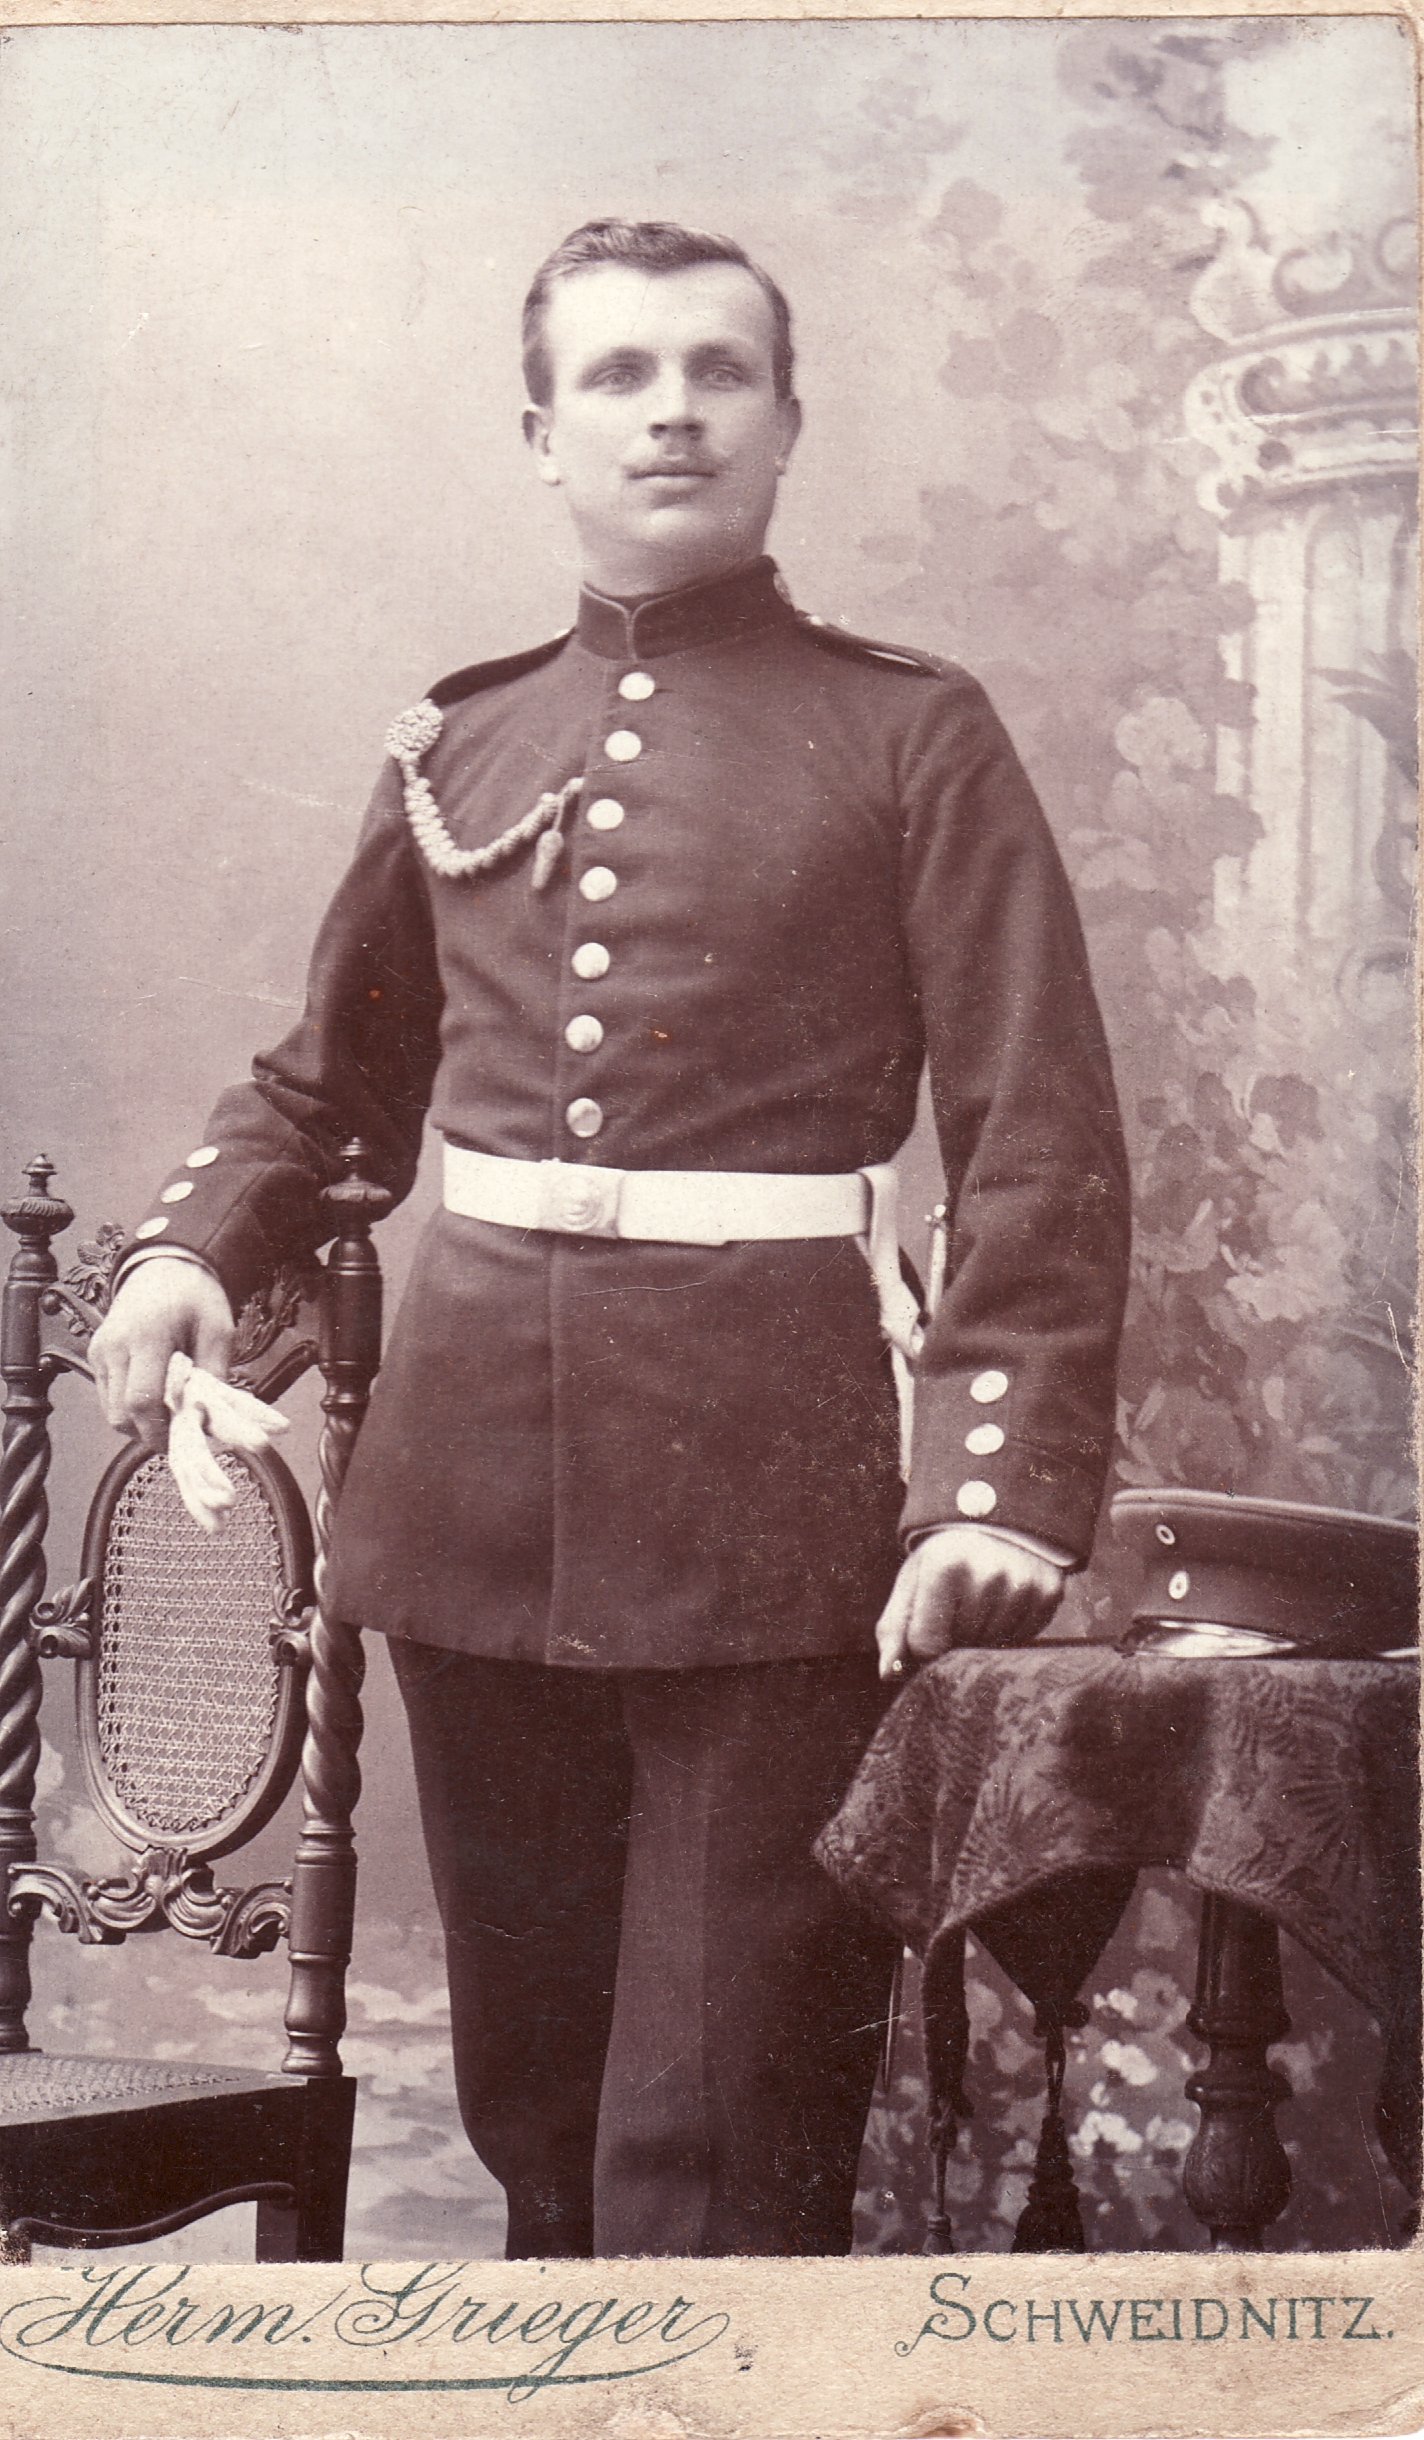
\includegraphics[width=0.55\textwidth]{photo/edward_swierczynski_1.jpg}
\caption[Edward Świerczyński]{Edward Świerczyński w mundurze pruskiej armii}
\end{center}
\end{figure}

Pierworodnym zaś był \textbf{Walenty}, który imię wziął po swym dziadku Walentym Świerczyńskim. Ów starszy brat Edwarda urodził się 1\textbf{3 lutego 1879 roku} także w \textbf{Łagiewnikach Wielkich}, w niecały miesiąc po ślubie swych rodziców, który odbył się 21 stycznia 1879 r. Trzecim i ostatnim ich dzieckiem był \textbf{Piotruś urodzony 25 czerwca 1889 r.} w Łagiewnikach Wielkich, który krótko żył, zmarł \textbf{5 marca 1892 r.}, w rok po śmierci swego ojca. Bowiem nasz \textbf{pradziadek Jan zmarł w wieku 39 lat w Łagiewnikach Wielkich 26 kwietnia 1891 r.} Wówczas nasz dziadek Edward miał niecałe 10 lat, jego starszy brat Walenty 12 lat, a ich matka Julia 41 lat. To musiał być straszny cios! Samotna kobieta z trójką dzieci... Jakoś sobie poradzili, ale Piotruś umarł.

\textbf{Walenty} w wieku 20 lat – \textbf{30 października 1899 r. w Łagiewnikach Wlk. pojął za żonę Juliannę Helios urodzoną 12 lutego 1878 r.} jako nieślubne dziecko \textbf{Katarzyny Helios} – służącej (ojciec nieznany – pewnie pan, u którego służyła jej matka Katarzyna, która też była nieślubnym dzieckiem). Owa Julianna poszła tropem mamusi, gdyż zanim wyszła za mąż \textbf{urodziła 17 maja 1898 r. nieślubne dziecko – Julię}. Ta nieślubna córka Julii – Julia młodsza wyszła 5 kwietnia 1921 r. w Koszęcinie za Karola Standenmajera. \textbf{Walenty Świerczyński} – brat naszego dziadka Edwarda poszedł w ślady swego ojca Jana i \textbf{ożenił się z Julianną Helios} – starszą od siebie o dwa lata panną z dzieckiem \textbf{30 października 1899 r. w Łagiewnikach Wielkich}. Można przypuszczać, że owo nieślubne dziecko było autorstwa Walentego, jeśli dajmy na to (co często los płata nieostrożnym kawalerom) owo dziecko swym lustrzanym podobieństwem ujawniało niezbicie, kto jest jego tatusiem. Więc Walenty chcąc nie chcąc dał się zaprowadzić przez swą Juliannę do ołtarza, jak onegdaj jego ojciec Jan! A musieli się śpieszyć, gdyż w dniu ślubu była już w szóstym miesiącu ze swą drugą córką \textbf{Marią, którą powiła 24 stycznia 1900 r.}

\begin{figure}[!h]
\begin{center}
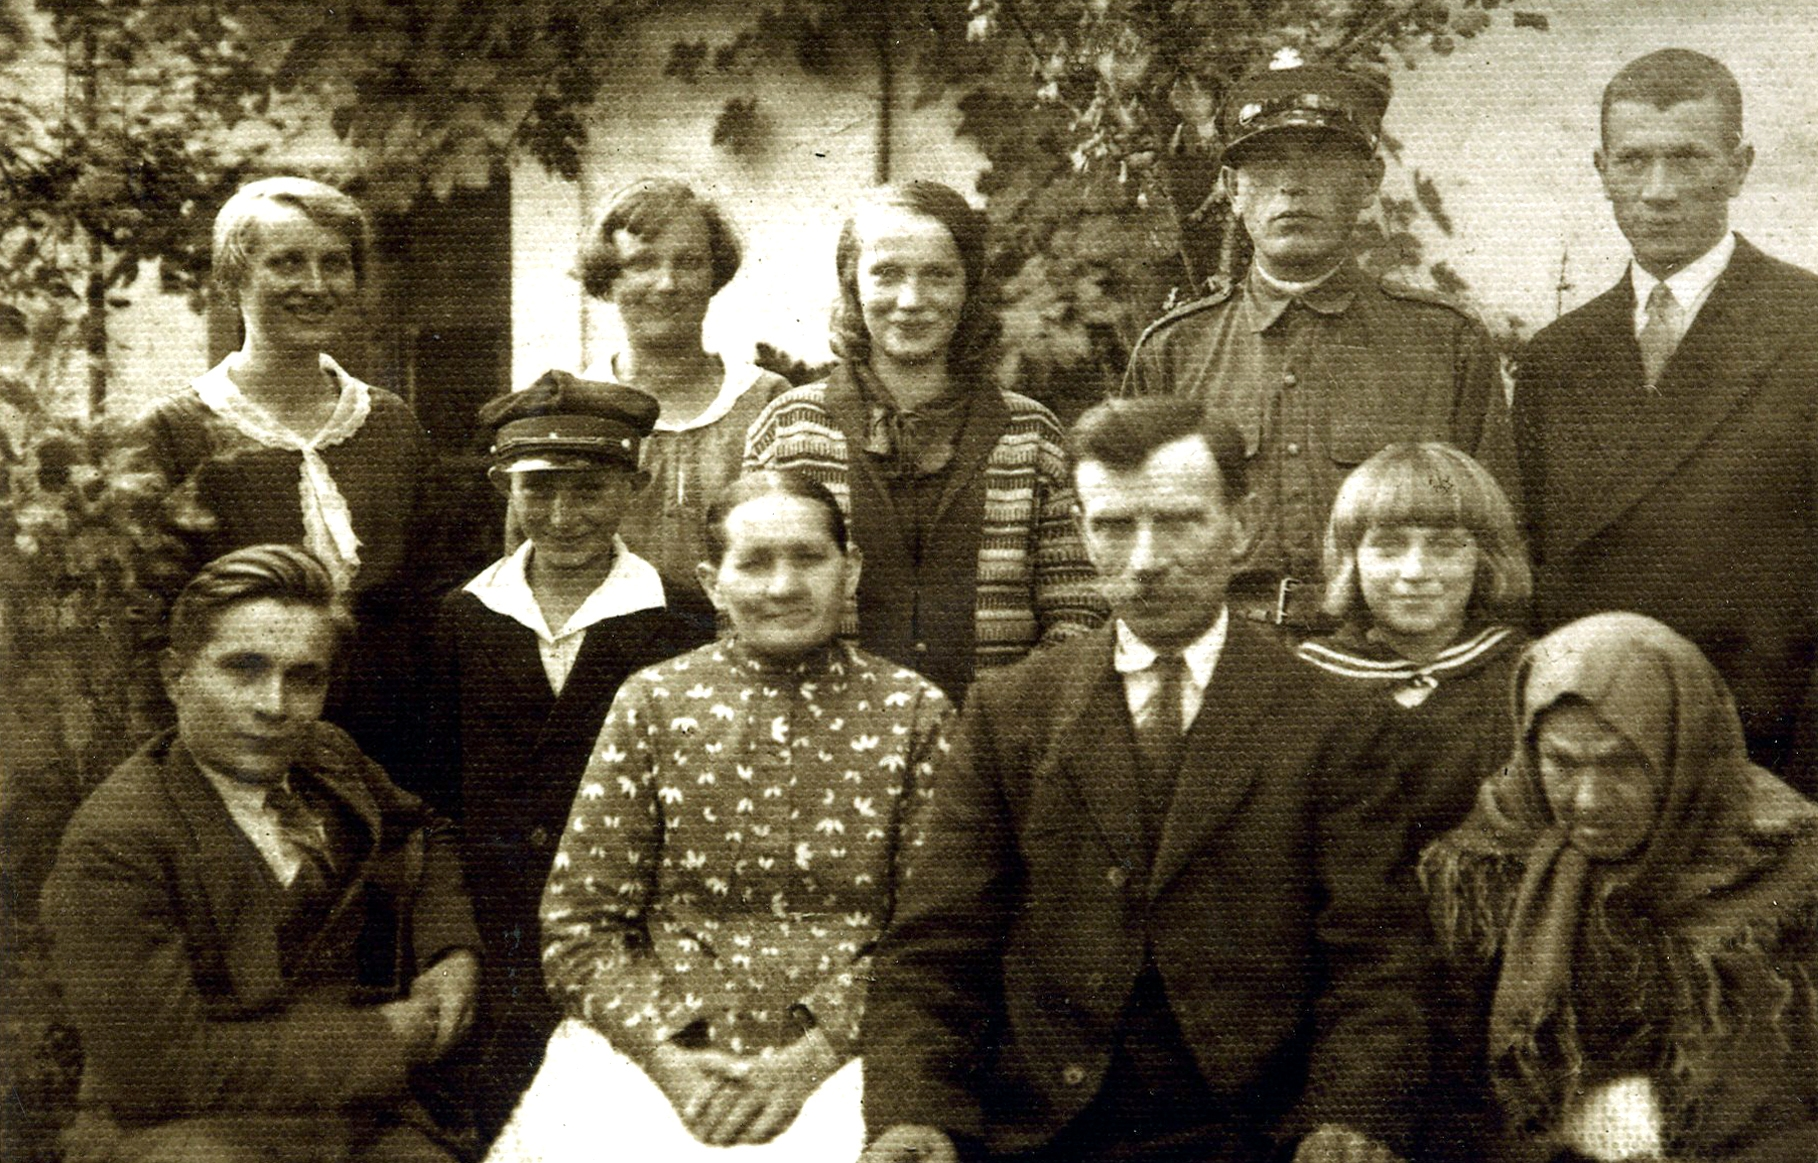
\includegraphics[width=\textwidth]{photo/rodzina_swierczynskich_1.jpg}
\caption[Rodzina Świerczyńskich z prababcią Julią]{Na zdjęciu rodzina Świerczyńskich: stoją od lewej: Anastazja, Benedykt (w czapce gimnazjalisty), Ludwika (żona Józefa), Irena, Karol i Józef, siedzą Wiktor, babcia Eufemia, dziadek Edward, za nim stoi Rózia, po prawej w chustce siedzi prababcia Julia Świerczyńska z domu Kępa.}
\end{center}
\end{figure}

Ileż wstydu podżyła nasza prababka Julia, bo przecież tylko ona wychowywała swoich synów, a pewnie we wsi dobrze pamiętali, że jej pierworodny Walenty też był „wcześniakiem” i to miesięcznym...\textbf{ W tym samym 1900 roku, lecz 27 grudnia} doczekali się młodzi małżonkowie \textbf{trzeciej córki – Agnieszki}. \textbf{27 lipca 1904 r.} przyszła na świat w Łagiewnikach Wielkich ich \textbf{czwarta córka – Anna}. \textbf{Dopiero 5 grudnia 1906 roku przyszedł na świat ich jedyny syn – Jan (wziął imię po swym dziadku)}, który – jak twierdziły śp. Stryjenki – Irena i Rózia – był niedorozwinięty, więc nie ożenił się. Walenty zatem nie doczekał się wnuka o nazwisku Świerczyński... \textbf{W 1908 r. – 7 grudnia} przyszła na świat \textbf{piąta ich córka, której nadali imię Maria}. Widocznie owa pierwsza Maria zmarła. \textbf{Ostatnim ich dzieckiem urodzonym w Łagiewnikach Wielkich była szósta córka Emilia, która przyszła na świat 7 maja 1911 r.} Wyszła ona 15 sierpnia 1933 r. za Władysława Parkitnego. Ostatnim ich dzieckiem, lecz urodzonym już w Koszęcinie, gdzie się przenieśli z całą rodziną, \textbf{była Franciszka urodzona 27 marca 1913 r.}

Przedstawiając ów najbardziej drastyczny obraz złamania nakazu czystości serc nowożeńców, chcę zwrócić uwagę czytelników niniejszej historii rodowej na bezwyjątkowy charakter reakcji Boga na ten grzech, czyli kary realizującej się na „owocu” owego przedmałżeńskiego współżycia, tj. na dziecku, z którego w każdym przypadku nie wyrosła męska gałąź kontynuacji rodu. Nie chcę tutaj wskazywać tych wszystkich „wcześniaków”, którzy przyszli na świat przed upływem 9 miesięcy od zawarcia małżeństwa. Najczęściej były to córki, które, jak wiadomo, nie kontynuują męskiej gałęzi rodu, a mimo to nie doczekały się własnego potomstwa, czy to dlatego, że nie wyszły za mąż, czy też dlatego, że Bóg ich nie obdarzył potomstwem. W przypadku chłopców „wcześniaków” najczęściej się oni nie ożenili, a ci co zawarli związek małżeński nie doczekali się potomstwa męskiego zdolnego kontynuować męską gałąź rodu, \textbf{co widać dobitnie na przykładzie owego Jana}, wnuka naszego pradziadka Jana i syna Walentego!!! Wiem to na podstawie historii czterech badanych przeze mnie rodów, tj. Świerczyńskich, Wilczków, Głąbów i Mertów.

Piszę o tym, by przestrzec Was Młodzi przed Bożym Gniewem... Dziecko płci męskiej poczęte przez Dawida w łonie ślicznej Batszeby, żony Uriasza Hetyty zaraz po powiciu umarło. Dopiero kolejne dziecko z tego związku – Salomon – okazało się następcą tronu królewskiego. Słynął on z mądrości do czasu, kiedy tych żon miał już wiele i z nimi zdradzał Boga Jahwe, oddając hołd bożkom przez nie wyznawanym... Do głupoty i głupich wyborów życiowych zawsze prowadzi nieuporządkowany seks! Bóg dlatego żąda małżeństw monogamicznych i pragnie czystości przedmałżeńskiej. Komu się chce, może sprawdzić, czy piszę prawdę...

\textbf{O swoim ojcu a naszym dziadku Edwardzie} tak pisze w swym pamiętniku mój ojciec – Benedykt : \textit{„\textbf{Ojciec mój kupił od Stanoska dom z chlewem kryty dachówką, szopę na zbiory, studnię w podwórku i osiem hektarów karczowiska i młodego lasu.} Był to chyba 1906 r. W to gospodarstwo wprowadził naszą Mamę i naszą Starkę. Z opowiadań Mamy wynikało, że Ojciec podjął decyzję przerastającą jego i rodzinki siły. Ziemia była licha, możliwej pod uprawę było 2 – 3 ha, reszta chaszcze, poręba, doły. Do dziś wiemy, co to są „lisie jamy” i skąd ta nazwa. Ta cała bieda jedną zaletę miała – była swoja, własna.''}

\begin{figure}[!h]
\begin{center}
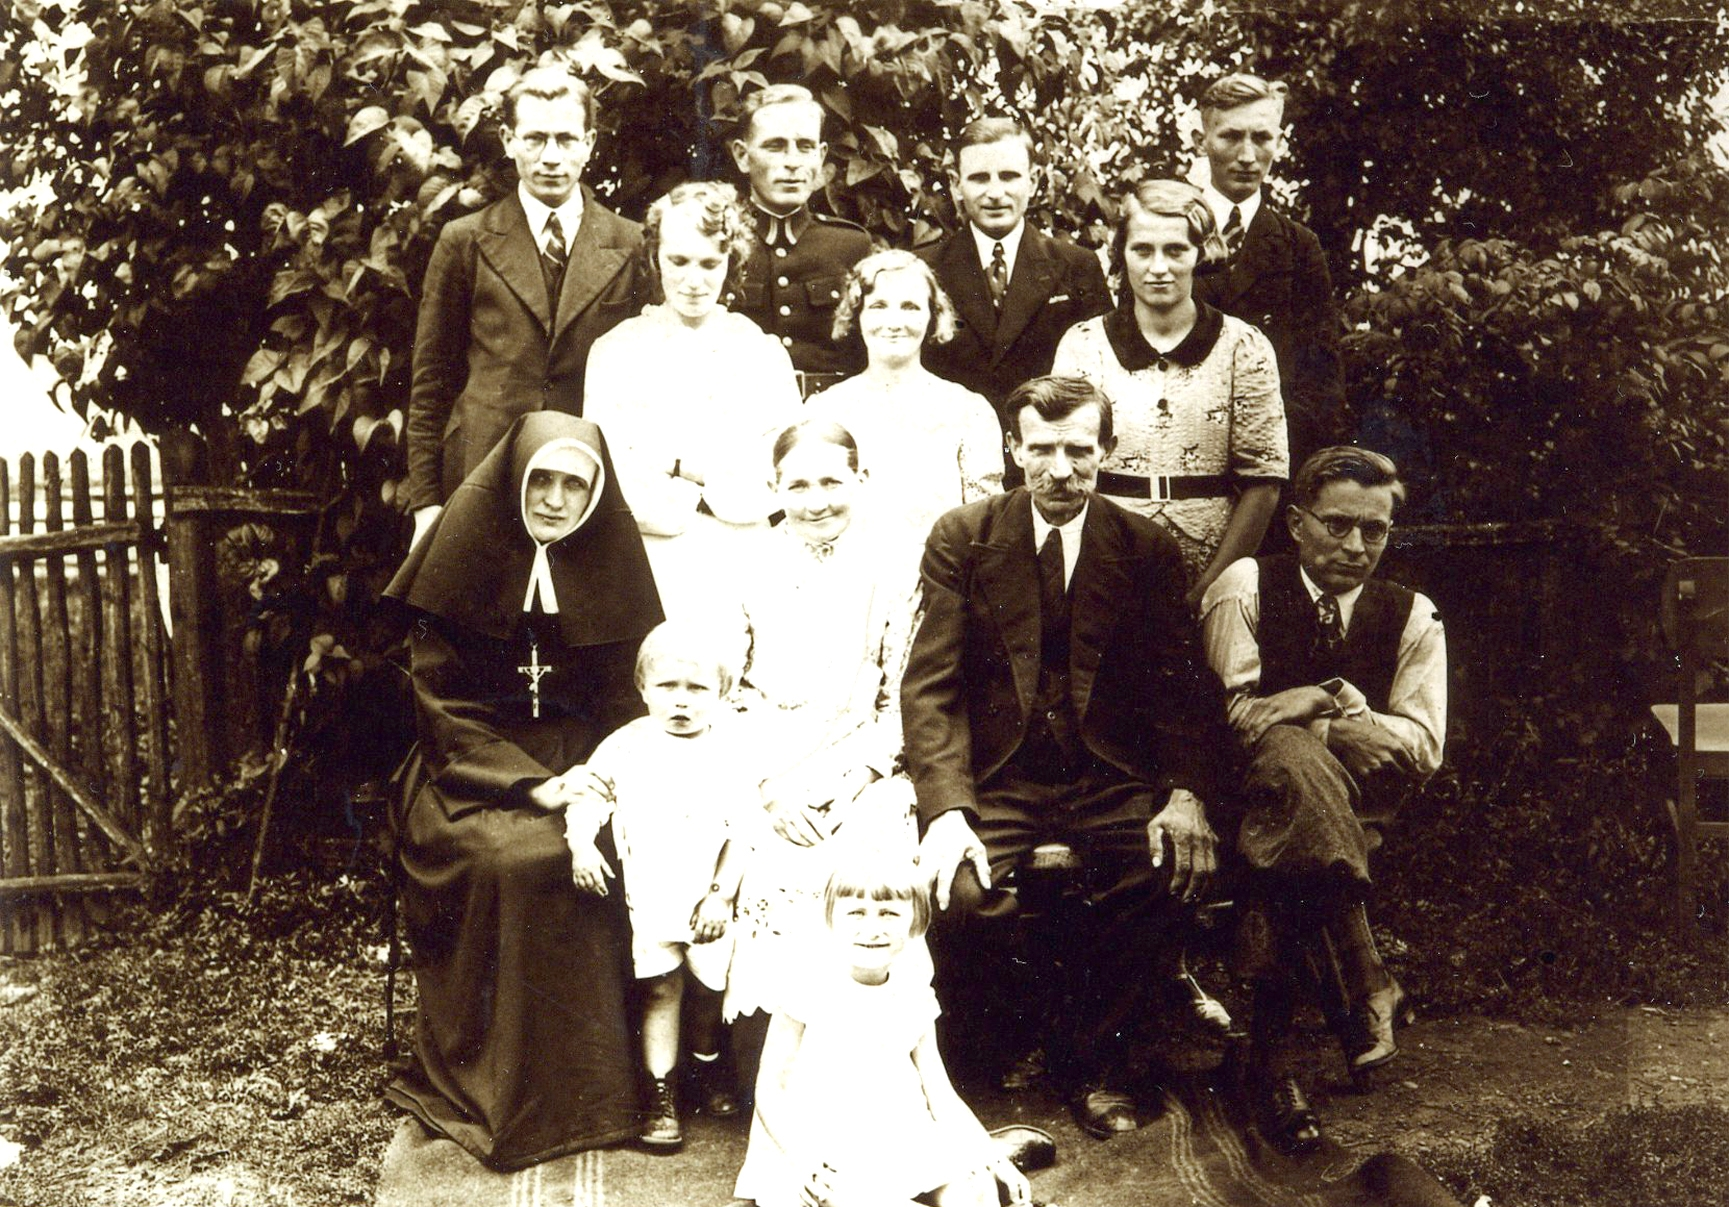
\includegraphics[width=\textwidth]{photo/rodzina_swierczynskich_2.jpg}
\caption[Rodzina Świerczyńskich z Wirgusiem]{Na zdj. siedzą od lewej: s. Aurelia Świerczyńska, Eufemia i Edward Świerczyńscy, Wiktor Świerczyński, przed nimi: Wirguś i Elżbieta Świerczyńscy, stoją w I rzędzie: Irena Lehman, Ludwika Świerczyńska i Róża Świerczyńska, w II rzędzie: Józef i Karol Świerczyńscy, Antoni Lehman (mąż Ireny) i Benedykt Świerczyński.}
\end{center}
\end{figure}

Jeśli do niej dodać fantazję Ojca – wizję przyszłości, niesłychaną pracowitość, jego dość wszechstronne zdolności i ambicję zostania „gospodarzem jak się patrzy” – można zrozumieć jak w ciągu  dwudziestu lat zaledwie (wyjąwszy 4 lata I wojny światowej) mógł zmienić się obraz tej całej biedy. To co ja widziałem na własne oczy i zdołałem zapamiętać nie bardzo mi pasowało do opowiadań Mamy czy starych sąsiadów o tym, jak to było pierwej. Bo na ten przykład pole było od miedzy do miedzy, od pańskiego lasu do lasu Kusiowego bez śladu poręby, a piaszczysta górka przed łąką już tylko nazywała się \textit{lisie jamy}.

Widok z okna na to pole zasłaniała stodoła, wysoka, z gumnem i dwoma sąsiekami, a te grube balki to było piętro i jeszcze wyżej to były bunty. To już było wysoko, że strach… Filary były murowane, ściany były z desek, a dach słomiany z głowoców. Kiedy Ojciec budował tę stodołę, stary Kuś pytał, podśmiewując się: Ejduś, co ty bedzieś do niej skłodoł, gałęzie z lasa? Aliści, kiedy miałem lat dziesięć, ta stodoła już była za mała, nie mieściła zboża, a pola przecież nie przybyło. Trzeba było stodołę poszerzać o przybudówki, a słomę ustawiać w bróg na polu. Podobnież było z „rurkowaniem” pola. \textit{Co ty robisz Ejduś} -- pytał stary Kuś – \textit{Jak przyjdzie suche lato, to ci nic nie urośnie, jak ty wodę z pola spuścisz, co bydziesz jod?} Ojciec zawierzył nowościom i całe pole zdrenował sam. Ile set metrów rowów melioracyjnych wykopał sam łopatą, ile rurek, tj. drenów położył, jak to spoziomował, że woda spływała jak trza, że w mokre lata nie było grzęzawisk, a w suche wilgotniej było niż na sąsiednim – Kusiowym polu – tego nie wiem. Wyobrażam sobie tylko, jak duża to była inwestycja i ile wymagała pracy mięśni i pomyślunku. Dzielny był nasz Ojciec i zdolny do wyrzeczeń. Nie złamały go „wypadki nadzwyczajne” i przeróżne nieszczęścia, których w swój i nasz życiorys nie wkalkulował, bo przecież nie mógł przewidzieć…

I wojna światowa zabrała mu pełne cztery lata. Miał jednak wielkie szczęście, bo spodobał się aptekarzowi frontowemu, więc wraz z nim wojował na dość bezpiecznych tyłach, chyba przez dwa lata, gdzieś na froncie wschodnim. Opowiadał coś o Polesiu, o Pińsku. Mniej mówił o froncie zachodnim, gdzie też był przez pewien czas. Ilekroć prosiliśmy o jakieś szczegóły, opisy, refleksje, zbywał nas brakiem czasu lub zdawkowymi epizodzikami z tych kampanii. Sam do tej tematyki nie nawiązywał nigdy w obecności dzieci. Zapytany, dlaczego nie chce opowiadać swych wojennych przygód, skwitował to następująco: „Dzieci, wy tego nigdy nie zrozumiecie, to trzeba przeżyć samemu, żeby zrozumieć grozę, okrucieństwo, przekleństwo wojny…”. 

\textbf{Nasza Babusia – Eufemia Grabińska, zwana „Ofką”, przyszła na świat 9 września 1883 r. w Łagiewnikach Wielkich jako druga córka Jakuba Grabińskiego i Zofii z domu Kępa.} Mój ojciec Benedykt tak o niej pisze w swoim pamiętniku: „Czy możecie sobie wyobrazić sytuację, w jakiej znalazła się nasza Mama, gdy Ojca zabrali na wojnę? Józef miał lat 7, Karol 5, Hyjka 3, Wiktor roczek, Starka 64 lata, a do tego pole i obórka (kilka ogonów) i koń ( na szczęście bardzo spokojny). Jak Oni sobie radzili, ile to kosztowało wyrzeczeń, pracy, zachodu, a przy tym ile obaw kiedy i czy wróci? Dla mnie pozostaje to do dziś tajemnicą jak, jakim kosztem zdrowia, pracy, nieprzespanych nocy i czym tam jeszcze dokonała tego, że pole było uprawione, zbiory zebrane, gadzina opatrzona, kontyngenty oddane, drwa narąbane, a dzieci głodem nie przymierały… Tak więc bez cienia przesady można powiedzieć, że nasza Mama również dzielną była, zaradną i podziwiam ją, że nigdy nie straciła pogody ducha, nawet wtedy, kiedy przyszły na nią jeszcze gorsze terminy. 

\begin{figure}[!h]
\begin{center}
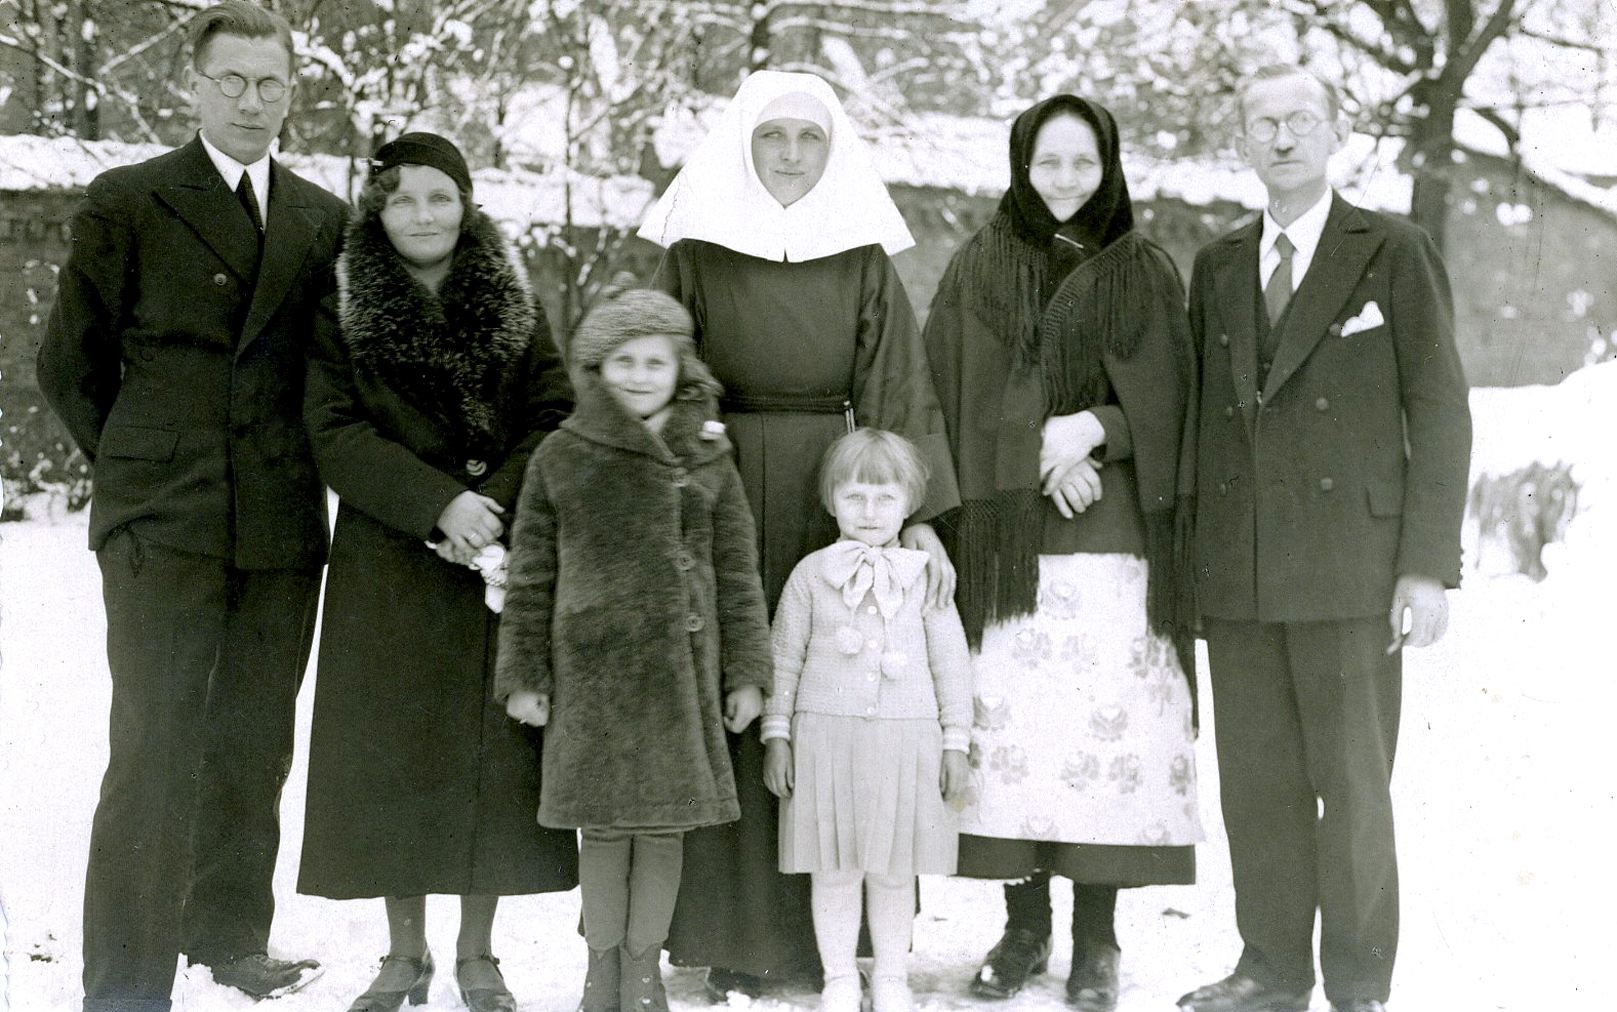
\includegraphics[width=\textwidth]{photo/eufemia_swierczynska.jpg}
\caption[Rodzina Józefa Świerczyńskiego z Janiną Grabińską]{Na zdj. od lewej: Józef i Ludwika Świerczyńscy, Janina Grabińska, s. Aurelia Świerczyńska, Ela Świerczyńska, Eufemia Świerczyńska i Y. Grabiński.}
\end{center}
\end{figure}

Miała Ona również pewne zasady, które nie kolidowały nigdy z jej prawdziwą pobożnością. Nie mogła się nigdy, dla przykładu, pogodzić z rozpowszechnianymi i praktykowanymi, zwłaszcza przez baby ze wsi, gusłami, zabobonami. Pouczała, że po pierwsze to jest grzech przeciw pierwszemu przykazaniu, a po drugie nic to nie pomoże, przeciwnie, może nawet zaszkodzić. Nie potrafiła też kogokolwiek oszukać, gdyż nie chciała, nawet w sprawach drobnych, bo to byłoby nieetyczne. Nie mogła zrozumieć jak można coś sprzedać jako dobre, wiedząc, że jest zepsute, sfałszowane, niedoważone.  Dlatego też trudno jej było wytłumaczyć postępek niejakiego Brzeziny, który gdzieś około 1930 r. sprzedał nam krowę chorą na gruźlicę (o czym wiedział) jako sztukę hodowlaną, wskutek czego wszystkie trzy krowy zachorowały i trzeba je było sprzedać za marne pieniądze. Na wsi – w gospodarstwie to katastrofa. To i podobne, nawet nie tak drastyczne oszukaństwa traktowała jako okradanie bliźniego.

\textit{Nie kradnij} -- jej zdaniem – nie dotyczyło tylko pospolitego rabunku, kradzieży, ale w ogóle wszelkich oszustw ze szkodą dla drugiego człowieka. Brzezinie wybaczyła, nie obnosiła po wsi naszej krzywdy, nie potrafiła co dzień okłamywać Boga mówiąc Jemu: \textit{i odpuść nam nasze winy, jako i my odpuszczamy…} I tak traktowała wszystkich, którzy wobec nas byli niesprawiedliwi. Wolała sobie popłakać, schować krzywdę w sobie… A cóż dopiero rozpowiadać o kimś złe rzeczy, co się sprzeciwiało przykazaniu: \textit{Nie mów fałszywego świadectwa…} Surowo przestrzegała zasady: \textit{Jeżeli nie widziałeś, nie widziałeś wyraźnie, jeśli nie słyszałeś, nie słyszałeś wyraźnie, a więc jeśli nie wiesz na pewno – nie mów!} Nie paplaj dalej niesprawdzonych wieści, bo one mogą komuś zaszkodzić, kogoś bardzo skrzywdzić, zhańbić na długie lata. Ludzie bywają straszni… Nie dość, że oczerniają, to jeszcze po drodze czynią z igły widły! Znali ludzie naszą Mamę od tej strony i dlatego do Niej z plotkami raczej nie przychodzili, a kto mimo wszystko od czasu do czasu kogoś tam próbował obmówić spotykał się z jednoznaczną ripostą. Chwała Jej za to!

Miała też nasza Mama niewzruszone zasady natury estetycznej i kulturalnej. Przede wszystkim czystość. \textbf{Łachy} – mawiała – \textit{mogą być połatane, ale nie brudne, naczynia zawsze starannie umyte}. Kiedy Ją zapytano \textit{jak ona to robi, że od niej np. masło jest zawsze tak smaczne} – odpowiadała, że mleko stoi zawsze w umytych naczyniach kamionkowych, a maśniczka zawsze jest myta przed i natychmiast po jej użyciu i nic więcej nie trzeba. I tak było ze wszystkim. Jedzenie było skromne, ale zawsze na czystym stole i każdy miał swoje naczynie. Wspominam to, bo bywałem tu i ówdzie na naszej wsi w porze jedzenia i wyznam, że nawet gdyby poprosili do stołu, nie byłbym jadł, bo by mi nie smakowało ze wspólnej misy, przy głośnym siorbaniu i w chmurze much…

Nasza Mama kochała kwiaty. Sadziła je i siała każdego roku w ogródku. A baby ze wsi pytały: \textit{Czy nie szkoda pracy i ziemi?} Prawda, dziwna to była wiocha, bo na przykład w sąsiednim Lubecku w tym czasie już niektóre gosposie współzawodniczyły o najładniejsze ogródki…\textit{ Patrząc w te kwiaty zapominam choć na chwilę o twardym losie, a ponadto przecież one nikogo nie skrzywdzą} – mawiała. Nie unosiła się, nie krzyczała i nie uderzyła nikogo z nas, chociaż się niejednemu z nas młodych coś tam czasami przytrafiło. Zganiła oczywiście, uprzedziła, że w przypadku braku poprawy jakieś tam będą konsekwencje. Kiedy jednak zdarzyło się coś bardziej drastycznego następowały gorzkie wymówki i rzecz najgorsza… Mamine łzy. Dla mnie w każdym razie ta kara była najcięższa ze wszystkich kar. Nie mogłem potem długo spojrzeć Mamie w oczy.

\begin{figure}[!h]
\begin{center}
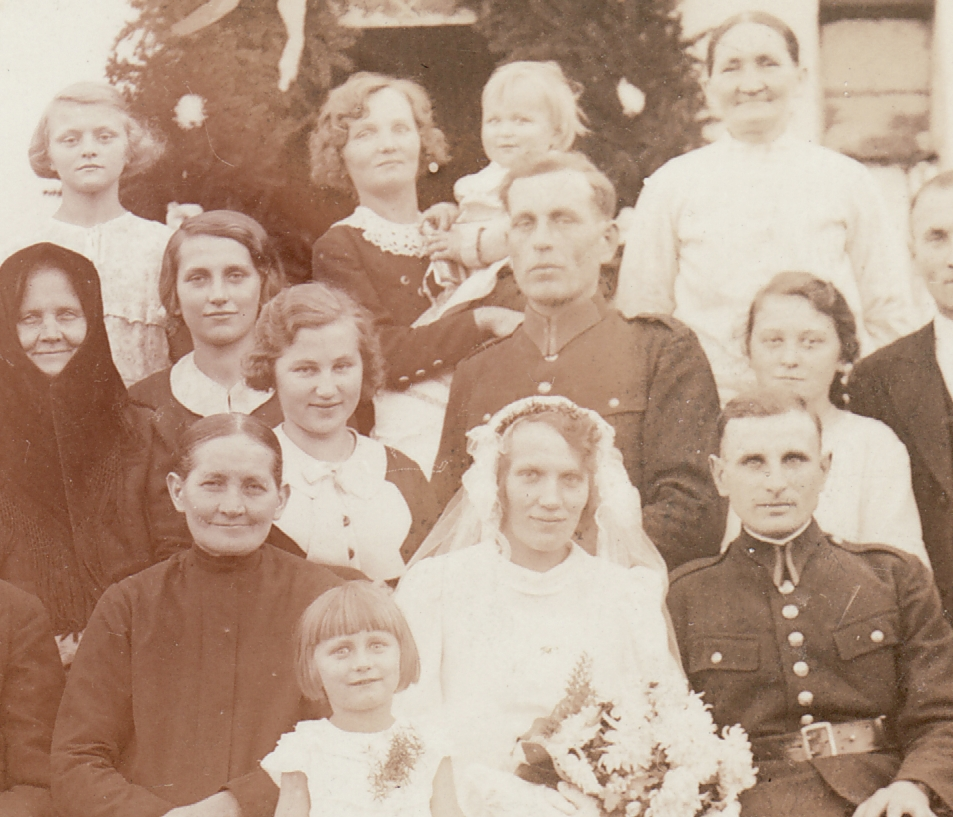
\includegraphics[width=0.6\textwidth]{photo/irena_antoni_lehman_slub_1.jpg}
\caption[Karol Świerczyński i Elżbieta Janik]{Karol Świerczyński i Elżbieta Janik -- stoją razem za stryjenką Ireną i babcią Eufemią (wycinek zdjęcia gości weselnych ze ślubu Ireny Świerczyńskiej i Antoniego Lehmana)}
\end{center}
\end{figure}

Przed Eufemią Grabińską – naszą „Babusią” \textbf{przyszła na świat 30 listopada 1881 r. w Łagiewnikach Wielkich – Maria Grabińska}, która wyszła za Jerzego (Jorga) Wąsa i miała z nim pięcioro dzieci (Marię Zofię, Zofię Marię, Jana, który dziedziczy ich gospodarstwo, Janinę i Edwarda, który zginął pod Berlinem). Po Eufemii, naszej Babusi, \textbf{przyszedł na świat 11 października 1885 r. Wiktor Grabiński}, który ożenił się z Franciszką Kroll na Rozbarku, gdyż na tamtejszej kopalni fedrował, później zaś kupił gospodarstwo na Zydlungu, w końcu gdy umarł, jego żona wróciła na Dębinę. Mieli trójkę dzieci: Helenę, Henryka i Lidię. Drugi syn Jakuba i Zofii – \textbf{Karol przyszedł na świat 3 listopada 1887 r.} Jego ojciec był wtedy murarzem. Karol Grabiński miał trójkę dzieci: syna Eryka, który gospodaruje w Łagiewnikach Wielkich, Eugenię mieszkającą obecnie w Lublińcu i już nieżyjącą Bronisławę. Wujek Karol jest na zdjęciu ślubnym naszej stryjenki Ireny i Antoniego Lehmanów. Siedzi obok Seweryny Lehman – matki stryja Antoniego, a po przeciwnej stronie tego rzędu stoi jego syn Eryk. Za stryjem Antonim stoi Bronisława – córka Karola, a w ostatnim rzędzie w drzwiach stoi Eugenia.

W trzy lata po Karolu \textbf{przyszła na świat Anna Grabińska, tj. 4 stycznia 1890 r.} Pewnie zmarła w wieku dziecięcym, skoro rodzina jej nie wymienia pośród dorosłych. W rok później \textbf{urodził się Edward Grabiński, tj. 20 września 1891 roku w Łagiewnikach Wielkich}. Był policjantem i mieszkał w Łagiewnikach koło Bytomia. Żenił się dwa razy. Najpierw 9 kwietnia 1948 r. w Kochłowicach z Gertrudą Oleksa, następnie z Marią Gąsior – wdową z domu Magiera, również w Kochłowicach. Mimo to umarł bezdzietnie. 
Najchwalebniej zapisał się w historii rodziny Jakuba i Zofii Grabińskich \textbf{ich czwarty syn Wincenty urodzony 10 stycznia 1894 r. w Łagiewnikach Wielkich}. Ożenił się w Krakowie Podgórzu z Jadwigą Grabińską, córką Andrzeja Grabińskiego i Urszuli z domu Respondek. Mieli ośmioro dzieci. Najstarszym – urodzonym w 1925 r. w Paruszowcu był Marian Grabiński, który został misjonarzem oblatem NMP we Francji. Tam się spotkał ze stryjem Józefem Świerczyńskim. Zmarł około 1998 r. we Francji. Po nim przyszła na świat w 1928 r. w Głogówku córka Helena, która w 1956 r. zmarła na Heine – Medina wkrótce po ukończeniu studiów magisterskich. W 1930 r. przyszedł na świat w Hajdukach – obecnie w Chorzowie Batorym, gdzie na stałe osiedli - ich drugi syn  - Zygmunt, który był księgowym, a ożeniwszy się z Wandą Kępińską miał z nią córkę Wiesławę. Zmarł w 2004 r. W Hajdukach 20 września 1932 r. przyszła na świat Janina Grabińska, która nie wyszła za mąż. Przez wiele lat – do emerytury była przewodnikiem turystycznym PTTK. Mieszka do dziś z bratem – starym kawalerem w Rybniku, w domku jednorodzinnym przy ul. Chełmońskiego 16a. Dzięki niej uzyskałem sporo informacji o późniejszych losach rodziny Grabińskich – braci i sióstr naszej babusi Eufemii. W dwa lata po Janinie 15 sierpnia w Hajdukach urodził się Czesław Grabiński, który ożenił się z Izabelą Manierą i ma z nią syna Aleksandra. Mieszkają w Chorzowie przy ul. Lompy 6. 8 lutego 1937 r. w Hajdukach przyszedł na świat Stefan Grabiński, który się nie ożenił i mieszka ze swą siostrą Janiną w Rybniku. 12 grudnia 1938 r. w Hajdukach Jadwiga Grabińska powiła bliźnięta: Bogusława i Aleksandrę. Bogusław ożenił się z Urszulą Szebesta, ma z nią córkę Bożenę, z którą mieszkają w Rybniku przy ul. Rynkowej 1. Aleksandra nie wyszła za mąż. Mieszka również w Rybniku przy ul. Św. Józefa 31c/42.

Wincenty Grabiński był przed wojną komisarzem policji, więc gdy hitlerowskie Niemcy napadły na Polskę uszedł wraz z Rządem RP przez Zaleszczyki do Rumunii, a stamtąd przez Jugosławię do Francji. Po upadku Francji w 1940 r. schronił się w Szwajcarii. Stamtąd wrócił w 1946 r. do Polski, więc go żydowskie UB zamknęło w więzieniu jako element klasowo wrogi PRL. Wyszedł z więzienia dopiero w 1956 r. Trzeba wielkiego samozaparcia i głębokiej wiary, by znając historię Polski nie stać się antysemitą!!!

Przedostatnim synem Jakuba i Zofii Grabińskich był \textbf{Konrad Emanuel urodzony 16 lutego 1896 r. w Łagiewnikach Wielkich}. Ożenił się 26 września 1922 r. z Augustyną Staniczek. Nie wiem czy mieli dzieci... \textbf{Najmłodszy syn i ostatnie dziecko Jakuba i Zofii to ur. 13 lutego 1901 r. Konstanty, Kostek Grabiński} zwany Kusztantem, który był księgowym w Hucie Kościuszko – mój chrzestny, który mnie widział tylko raz – podczas chrztu... Ożenił się 26 kwietnia 1951 r. z Gertrudą Rzeźniczek. Umarł bezdzietnie. Moim chrzestnym miał być wujek Walery i szkoda, że mój Tato w ostatniej chwili zmienił decyzję i zamiast niego został nim stryj Konstanty. \textbf{Jakub Grabiński ożenił się z Zofią Kępą w Lubecku 27 lutego1881 r. Miał z nią dziewięcioro dzieci. Zmarł w Łagiewnikach Wielkich  1 lipca 1916 r. w wieku 63 lat, a jego żona Zofia zmarła 3 listopada 1919 roku, mając 61 lat.}
\begin{figure}[!h]
\begin{center}
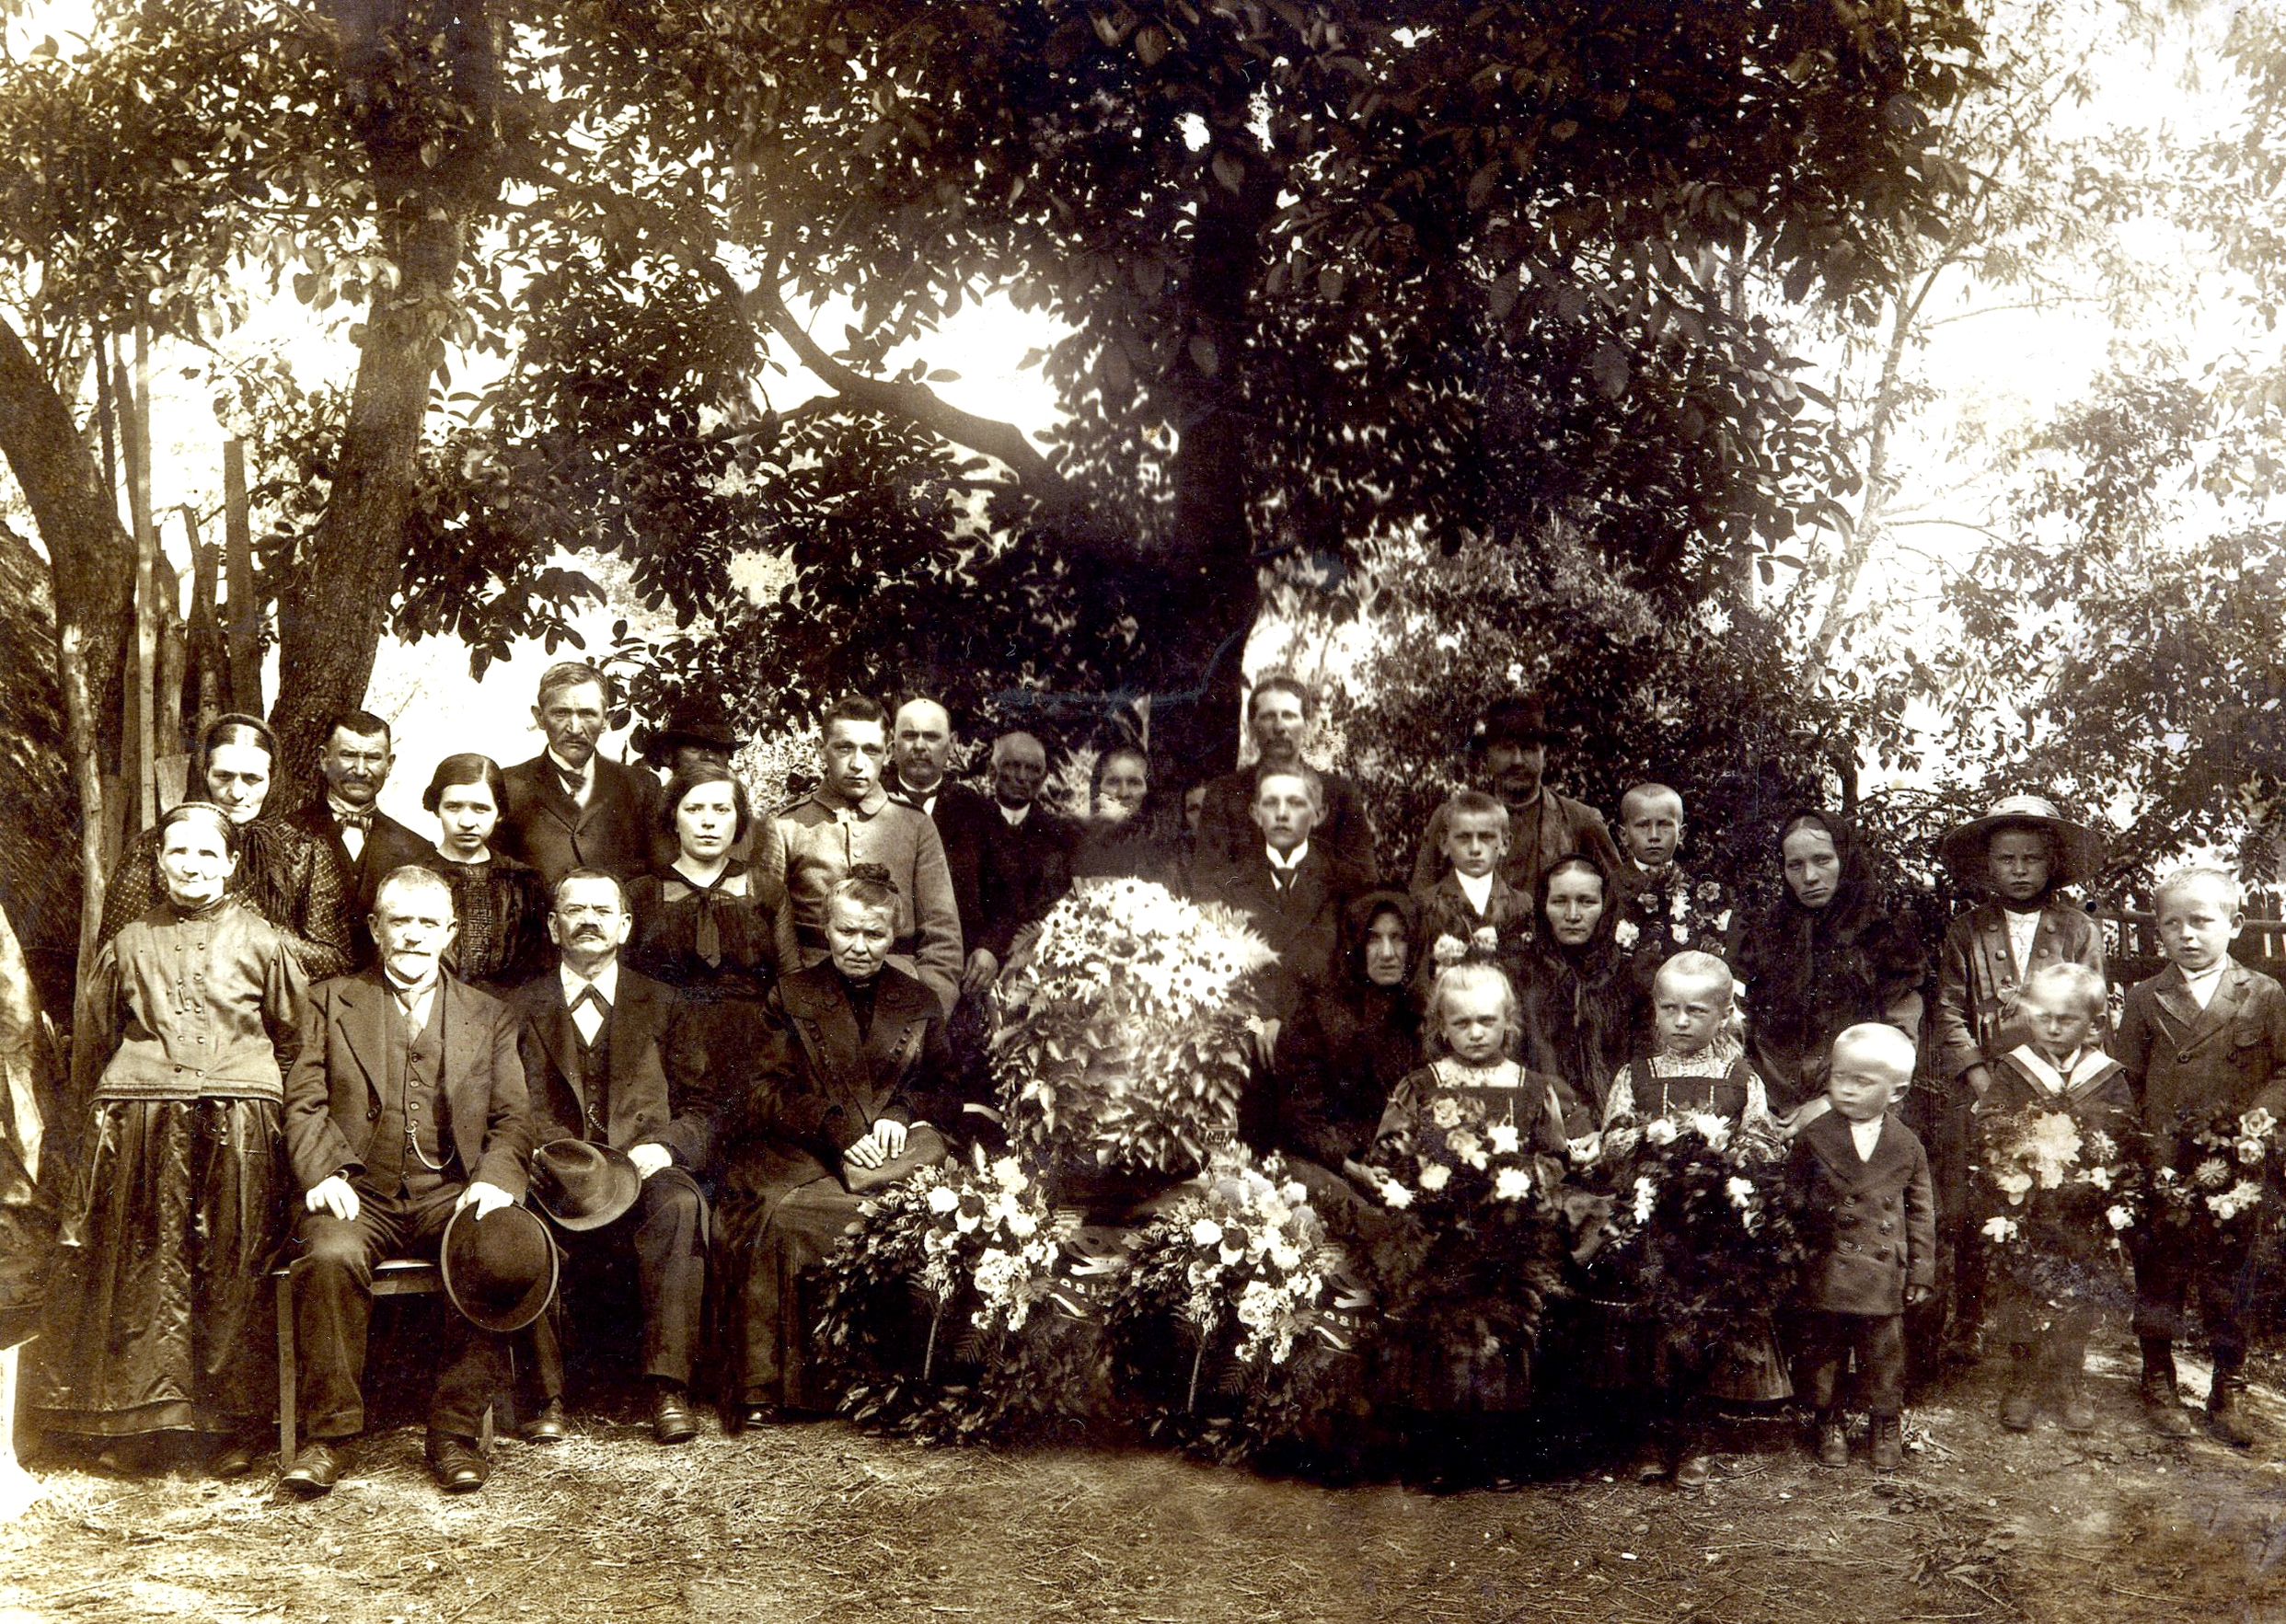
\includegraphics[width=\textwidth]{photo/jakub_grabinski_pogrzeb.jpg}
\caption[Pogrzeb Jakuba Grabińskiego]{Pogrzeb Jakuba Grabińskiego zmarłego w 1 VII 1916~r.}
\end{center}
\end{figure}

Mój prapradziadek Walenty urodził się w Panoszowie z Piotra Świerczyńskiego i Małgorzaty Konowoł dnia 13 lutego 1827 r. Ponoszów, czy Panoszów koło Sierakowa Śląskiego, to wioska o tradycjach hutniczych zwana do końca XVIII wieku Kuźnicą Sierakowską. Być może ojciec Walentego – Piotr Świerczyński był, jak później jego syn – woźnicą, stangretem, być może na służbie u właścicieli Kuźnicy. Właścicielami Panoszowa byli hrabiowie Kościelscy (ciekawe, czy mówili jeszcze po polsku?).

\begin{figure}[!h]
\begin{center}
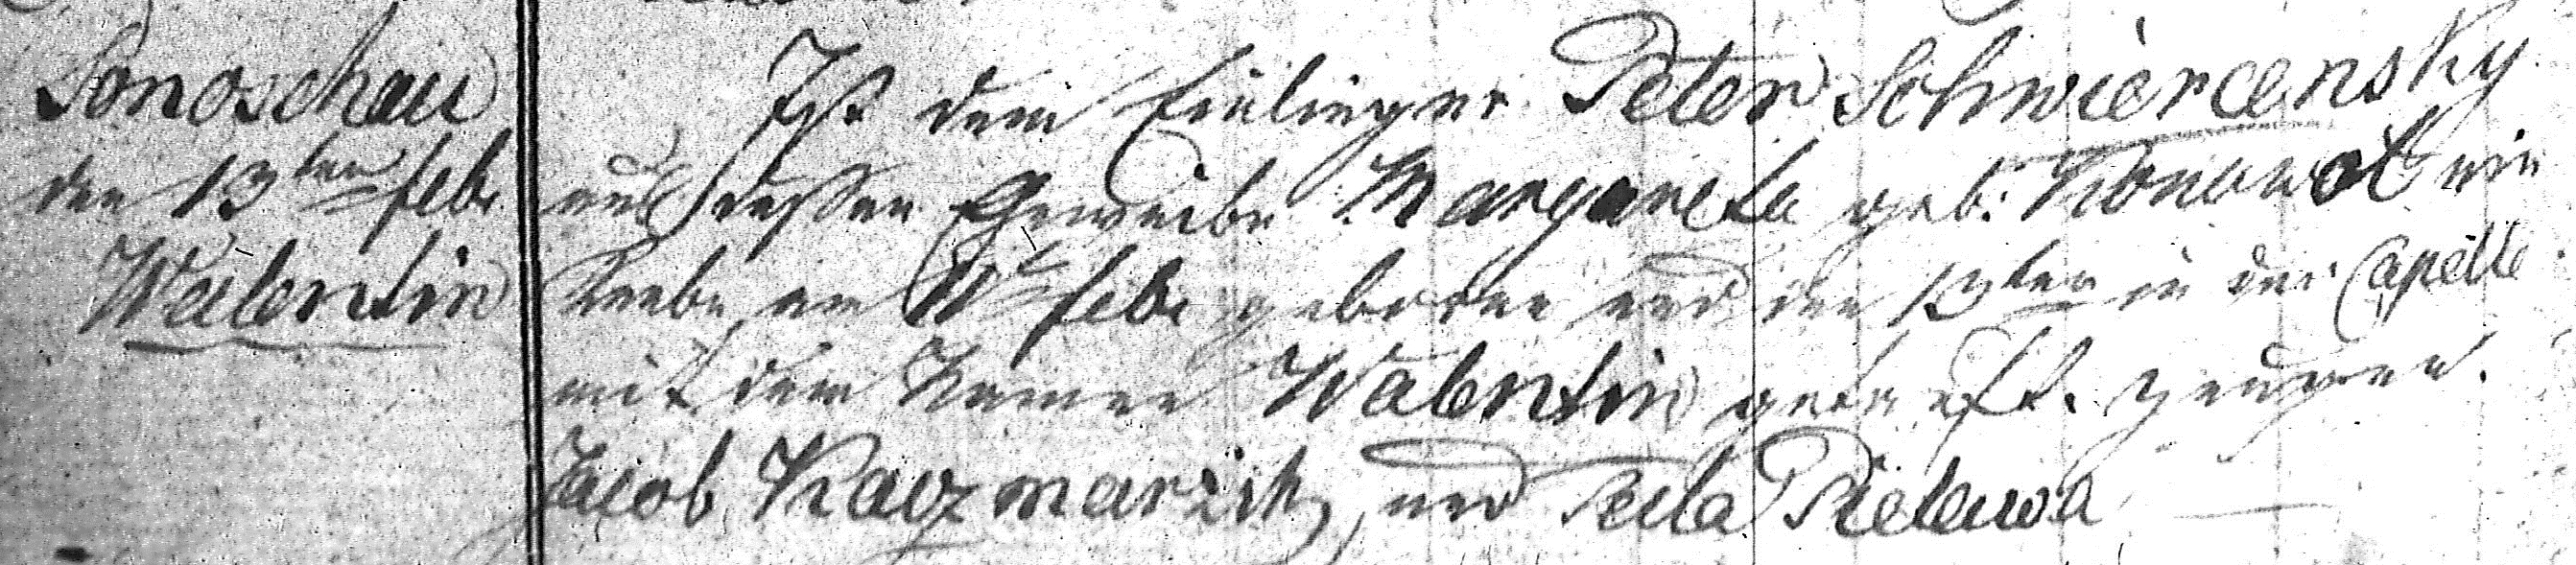
\includegraphics[width=\textwidth]{photo/ksiega_metrykalna_1.jpg}
\caption{Wyciąg z Księgi metrykalnej urodzenia Walentego Świerczyńskiego, syna Piotra.}
\end{center}
\end{figure}

W związku z tym, że pierwszym znanym mi (na razie)  protoplastą rodu Świerczyńskich okazał się Piotr, proponuję tytuł dla całej historii rodziny: „Od Piotra Pierwszego do Piotra Ostatniego”, lecz ten ostatni wcale nie jest taki ostatni, więc może ...do Piotra Współczesnego. Najlepiej  chyba będzie nawiązać do zdarzenia, które skłoniło mnie do sfinalizowania niniejszej edycji i nadać jej tytuł „Od Piotra Starego do Piotra Młodego. Dzieje siedmiu pokoleń Świerczyńskich”. 

\textbf{Walenty Świerczyński ożenił się  w Sierakowie z Zuzanną Nowok,} panną z Sierakowa – \textbf{8 września 1850 r. w kościele Piotra i Pawła.}
\begin{figure}[!h]
\begin{center}
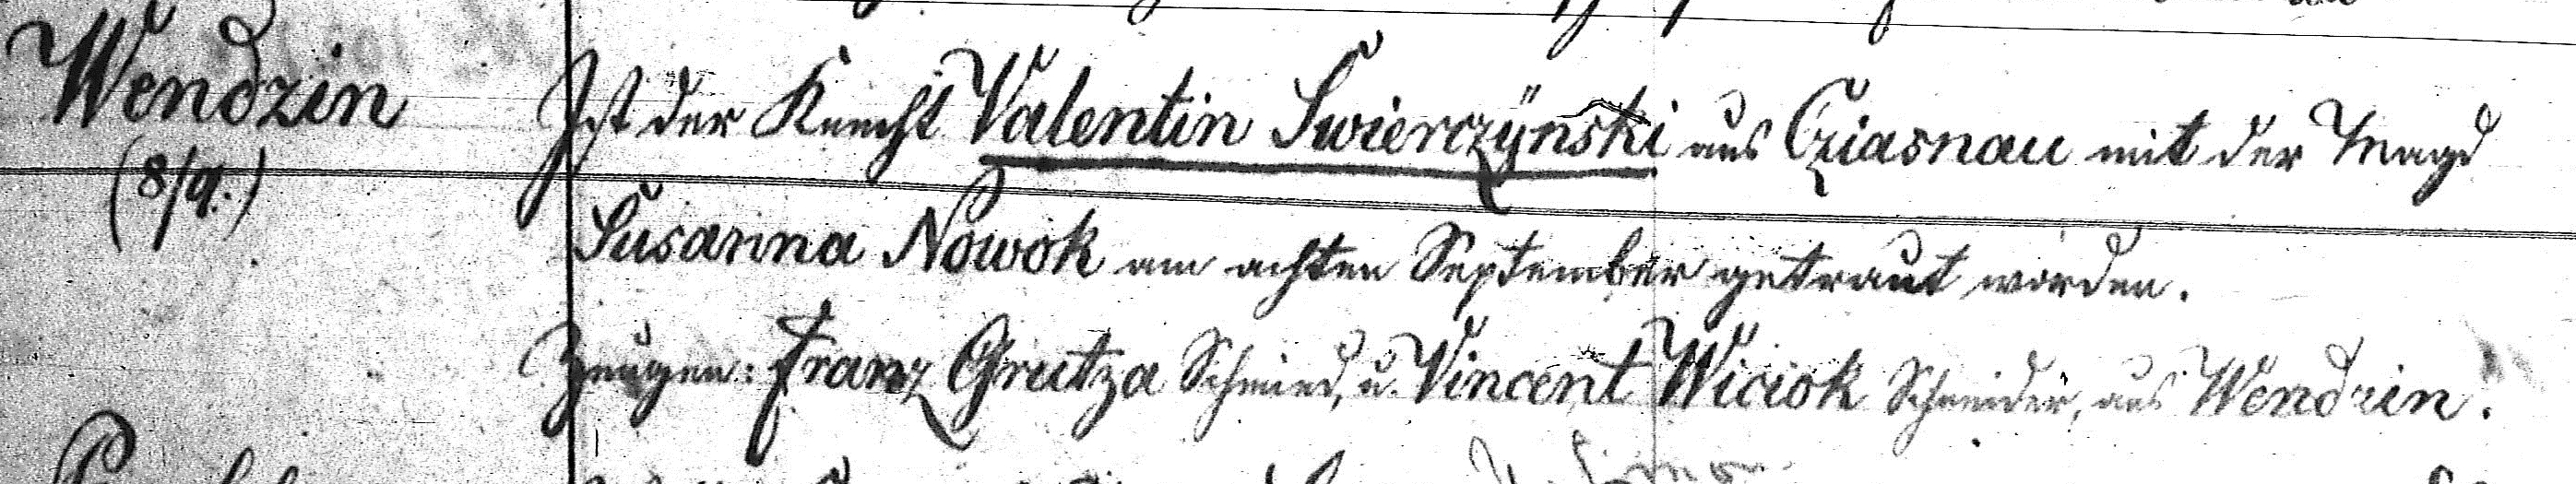
\includegraphics[width=\textwidth]{photo/ksiega_metrykalna_2.jpg}
\caption{Wyciąg z Księgi ślubów aktu ślubu Walentego Świerczyńskiego z Zuzanną Nowok}
\end{center}
\end{figure}

\textbf{Zuzanna była córką Macieja Nowoka i Marii Knietsch i przyszła na świat 31 lipca 1828 r. w Sierakowie.}
\begin{figure}[!h]
\begin{center}
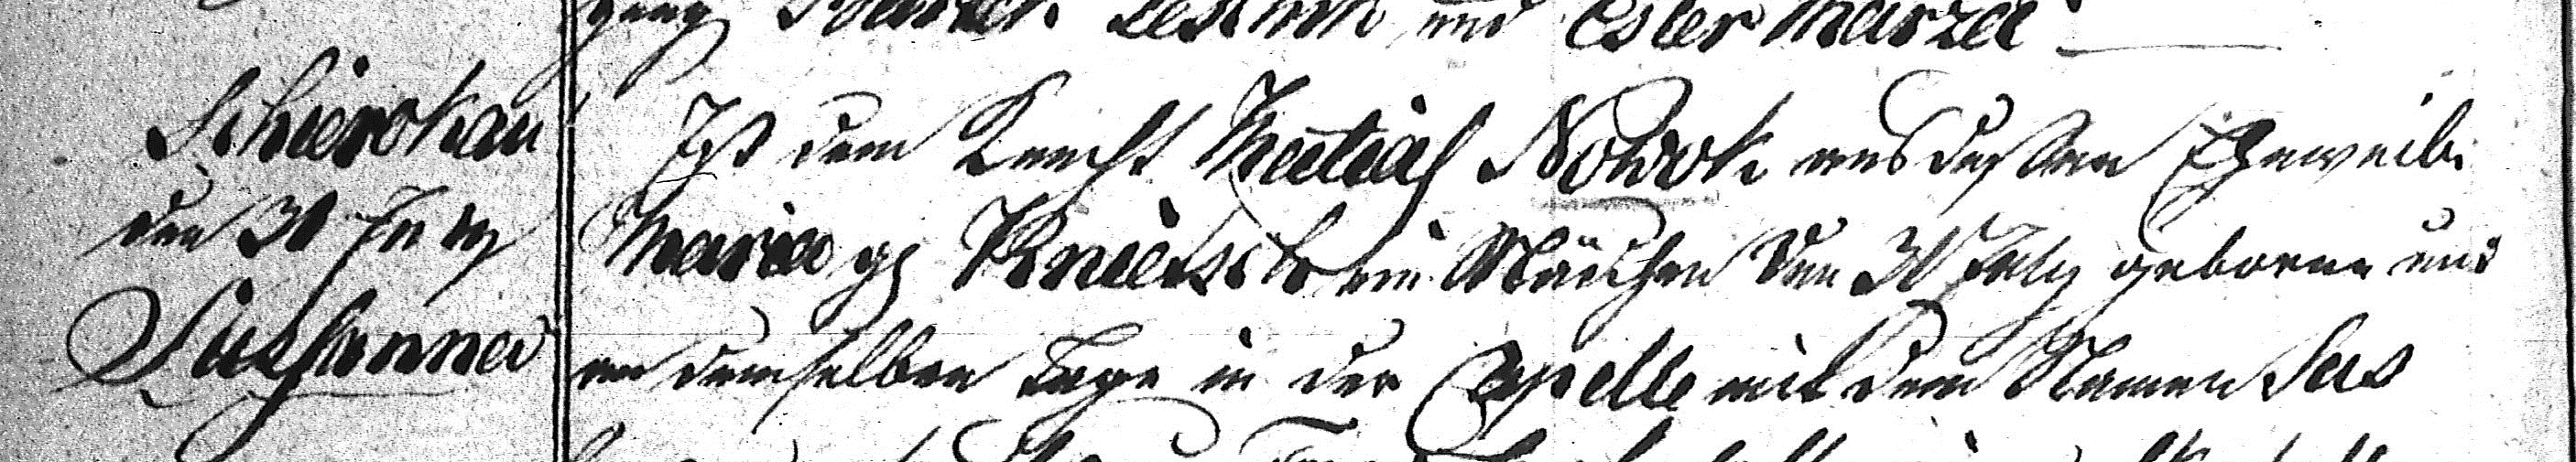
\includegraphics[width=\textwidth]{photo/ksiega_metrykalna_3.jpg}
\caption{Wyciąg z księgi metrykalnej urodzenia Zuzanny Nowok -- córki Macieja (Matiasa)}
\end{center}
\end{figure}


\begin{figure}[!h]
\begin{center}
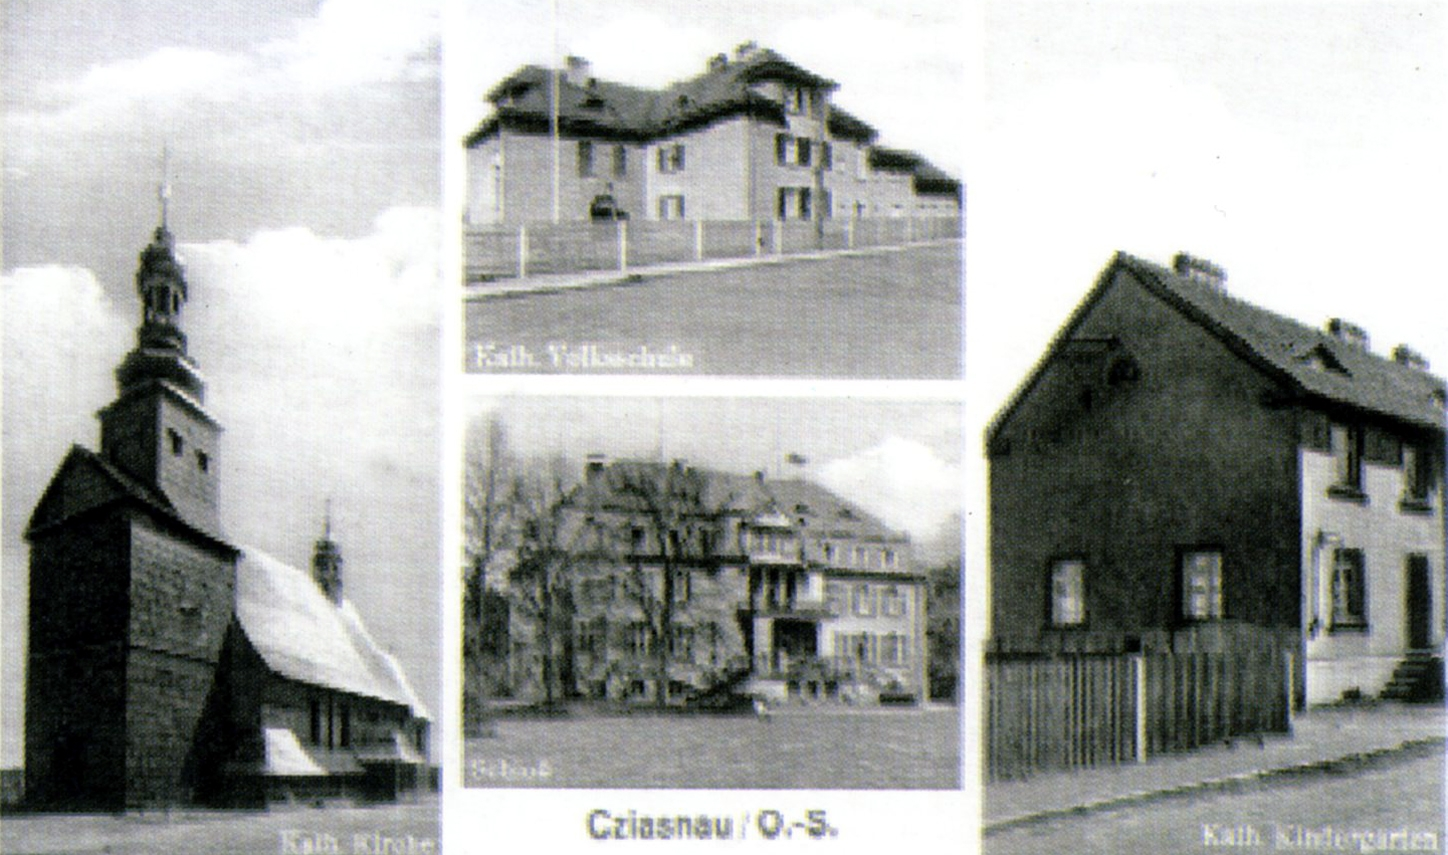
\includegraphics[width=0.7\textwidth]{photo/ciasno.jpg}
\caption[Ciasno]{Ciasno -- miejscowość rodzinna Walentego Świerczyńskiego i jego dzieci}
\end{center}
\end{figure}

Mieli ze sobą siedmioro dzieci: \textbf{Jana urodzonego 17 grudnia 1852 r. w Cieśnie, Agnieszkę Marię urodzoną 17 stycznia 1855 r., Pawła urodzonego 25 stycznia 1856 r., Ignacego Błażeja urodzonego 30 stycznia 1858 r. oraz Karola urodz. 18 maja 1859 r. jak i poprzedni w Cieśnie}. \textbf{5 sierpnia 1863 r. przyszła na świat Rosalia Świerczyńska, ale  już w Glinicy.} Po niej przyszedł na świat \textbf{10 marca 1866 r. Józef,} już jako syn wójta Gminy Glinica. Niestety, w cztery lata później już nie żył. Był to ostatni potomek Walentego i Zuzanny Świerczyńskich.

Moja Babcia Eufemia wywodzi się z rodziny Jakuba Grabińskiego i Zofii z domu Kempa. Ojciec babci Eufemii, czyli mój pradziadek Jakub był także synem Jakuba Grabińskiego i Józefy z domu Skiba, jako ich trzecie dziecko. Przed nim na świat przyszedł \textbf{15 stycznia 1848 r. w Łagiewnikach Wielkich – Antoni Grabiński}. Po nim \textbf{10 maja 1849 r. także w Łagiewnikach}, jak wszystkie ich dzieci – urodziła się \textbf{Joanna}, po niej zaś 15 \textbf{lipca 1853 r.} wspomniany wyżej \textbf{Jakub}, mój pradziadek. \textbf{17 września 1855 r.} rodzi się \textbf{Franciszek Grabiński}, po nim \textbf{13 sierpnia 1857 r.} przychodzi na świat \textbf{Ludwik}, a w dwa lata później \textbf{21 września 1859 r. Mateusz Grabiński} i w rok po nim \textbf{26 listopada 1860 r.} rodzi się \textbf{Andrzej Grabiński}. Po sześciu synach nareszcie dwie córki: najpierw \textbf{Julia Grabińska} urodzona \textbf{3 maja 1861 r.} a następnie \textbf{Krystyna} 	urodzona \textbf{10 czerwca 1864 r.} W rok później przychodzi na świat ostatnie ich dziecię – syn \textbf{Wawrzyniec (Lorenc) 9 sierpnia 1865 r.} \textbf{Jakub Grabiński} – ojciec wyżej wymienionych dziesięciorga dzieci, a mój prapradziadek przyszedł na świat \textbf{20 lipca 1815 r. w Łagiewnikach Wielkich} jako syn również \textbf{Jakuba Grabińskiego}, mojego praprapradziadka i \textbf{Zofii z domu Witzig}, mojej prapraprababki.

Każdy z nas ma dwoje rodziców, czworo dziadków ( tzn. dwóch dziadków i dwie babcie) , ośmioro pradziadków, szesnaścioro prapradziadków oraz  po szesnaście prapraprababć  i praprapradziadków. Ponieważ historia rodziny Świerczyńskich obejmuje tylko czwartą część całej waszej  rodziny moi  kuzynowie, więc wymienimy tutaj dla porządku tylko jednego dziadka i jedną babcię, dwóch pradziadków i dwie prababcie itd. Oto ich zestawienie:


1.Dziadkowie: 
  Edward Świerczyński ur. 11 X 1881 r. w Lublińcu; zm. 19 IX1945 r. w Łagiewnikach Wielkich;
  Eufemia Grabińska Świerczyńska ur. 9 IX 1883 r. w Łagiewnikach Wielkich, zm. 10 I 1951 r. w Łagiewnikach Wielkich;
2.Pradziadkowie:
  a) Jan Świerczyński ur. 17 XII 1852 r. w Cieśnie, zm. 26 IV 1891 r. w Łagiewnikach Wielkich;
  b) Julia Kępa Świerczyńska ur. 9 II 1850 r. w Łagiewnikach Wielkich; zm. 30 V 1933 r. w Łagiewnikach Wielkich;
  c) Jakub Grabiński ur. 15 VII 1853 r. w Łagiewnikach Wlk.; zm. 1 VII 1916 r. w Łagiewnikach Wielkich;          
  d) Zofia Kępa Grabińska ur. 13 V 1858 r. w Łagiewnikach Wielkich; zm. 3 XI 1919 r. w Łagiewnikach Wielkich;
3.Prapradziadkowie:
a) Walenty Świerczyński ur. 13 II 1827 r. w Panoszowie; zm. 26 IX 1885 r. w Cieśnie;
b) Zuzanna Nowok Świerczyńska ur. 31 VII 1828 r. w Sierakowie Śl.;
c) Andrzej Kępa ur. 3 III 1819 r. w Łagiewnikach Wielkich;
d) Maria Kandysch Kępa ur. 7 VI 1824 r. w Łagiewnikach Wielkich;
e) Jakub Grabiński ur. 20 VII 1815 r. w Łagiewnikach Wielkich;
f) Józefa Skiba Grabińska ur. 26 II 1824 r. w Cieśnie; zm. 4 XI 1893 r. w Łagiewnikach Wielkich;
g) Grzegorz Kępa ur. 22 XI 1818 r. w Molnej;
h) Janina Tomala Kępa ur. 11 VII 1814 w Lisowicach;
4.Praprapradziadkowie:
a) Piotr Świerczyński,
b) Małgorzata Konowoł Świerczyńska,
c) Maciej Nowok,
d) Maria Kniesch Nowok,
e) Bernard Kępa, 
f)  Katarzyna Polok Kępa,
g) Jakub Kandysch,
h) Maria Zowada Kandysch,
i) Jakub Grabiński,
j) Zofia Witzig Grabińska,
k) Karol Skiba,
l) Jadwiga Skubała Skiba,
m) Bartek Kempa (Kępa),
n) Zofia Bonk (Bąk) Kępa,
o) Antoni Tomala,
p) Józefa Smolin,

Jak widzicie, Drodzy Moi, jeszcze sporo pracy czeka tych, którzy wejdą w mój trud zebrania i odkrycia ważnych faktów dotyczących historii rodziny Świerczyńskich. Podejmijcie ten trud, to naprawdę pasjonująca przygoda, a księgi metrykalne sięgają nawet końca XVII w.  Powodzenia! 

\begin{flushright}
Czesław Świerczyński
syn Benedykta i wnuk Edwarda, oraz prawnuk Jana, 
praprawnuk Walentego oraz prapraprawnuk Piotra Świerczyńskiego.
\end{flushright}














\clearpage

PS: \textit{Szczególne wyrazy podziękowania za pomoc przy realizacji tej edycji należą się Małgosi Sojce i Ojcu Oskarowi za zeskanowanie kilkuset zdjęć, a także Piotrusiowi i jego Justynie oraz Krzysiowi Kordusowi, a zwłaszcza redaktorowi technicznemu – Bożydarowi Świerczyńskiemu.}

\begin{figure}[!h]
\begin{center}
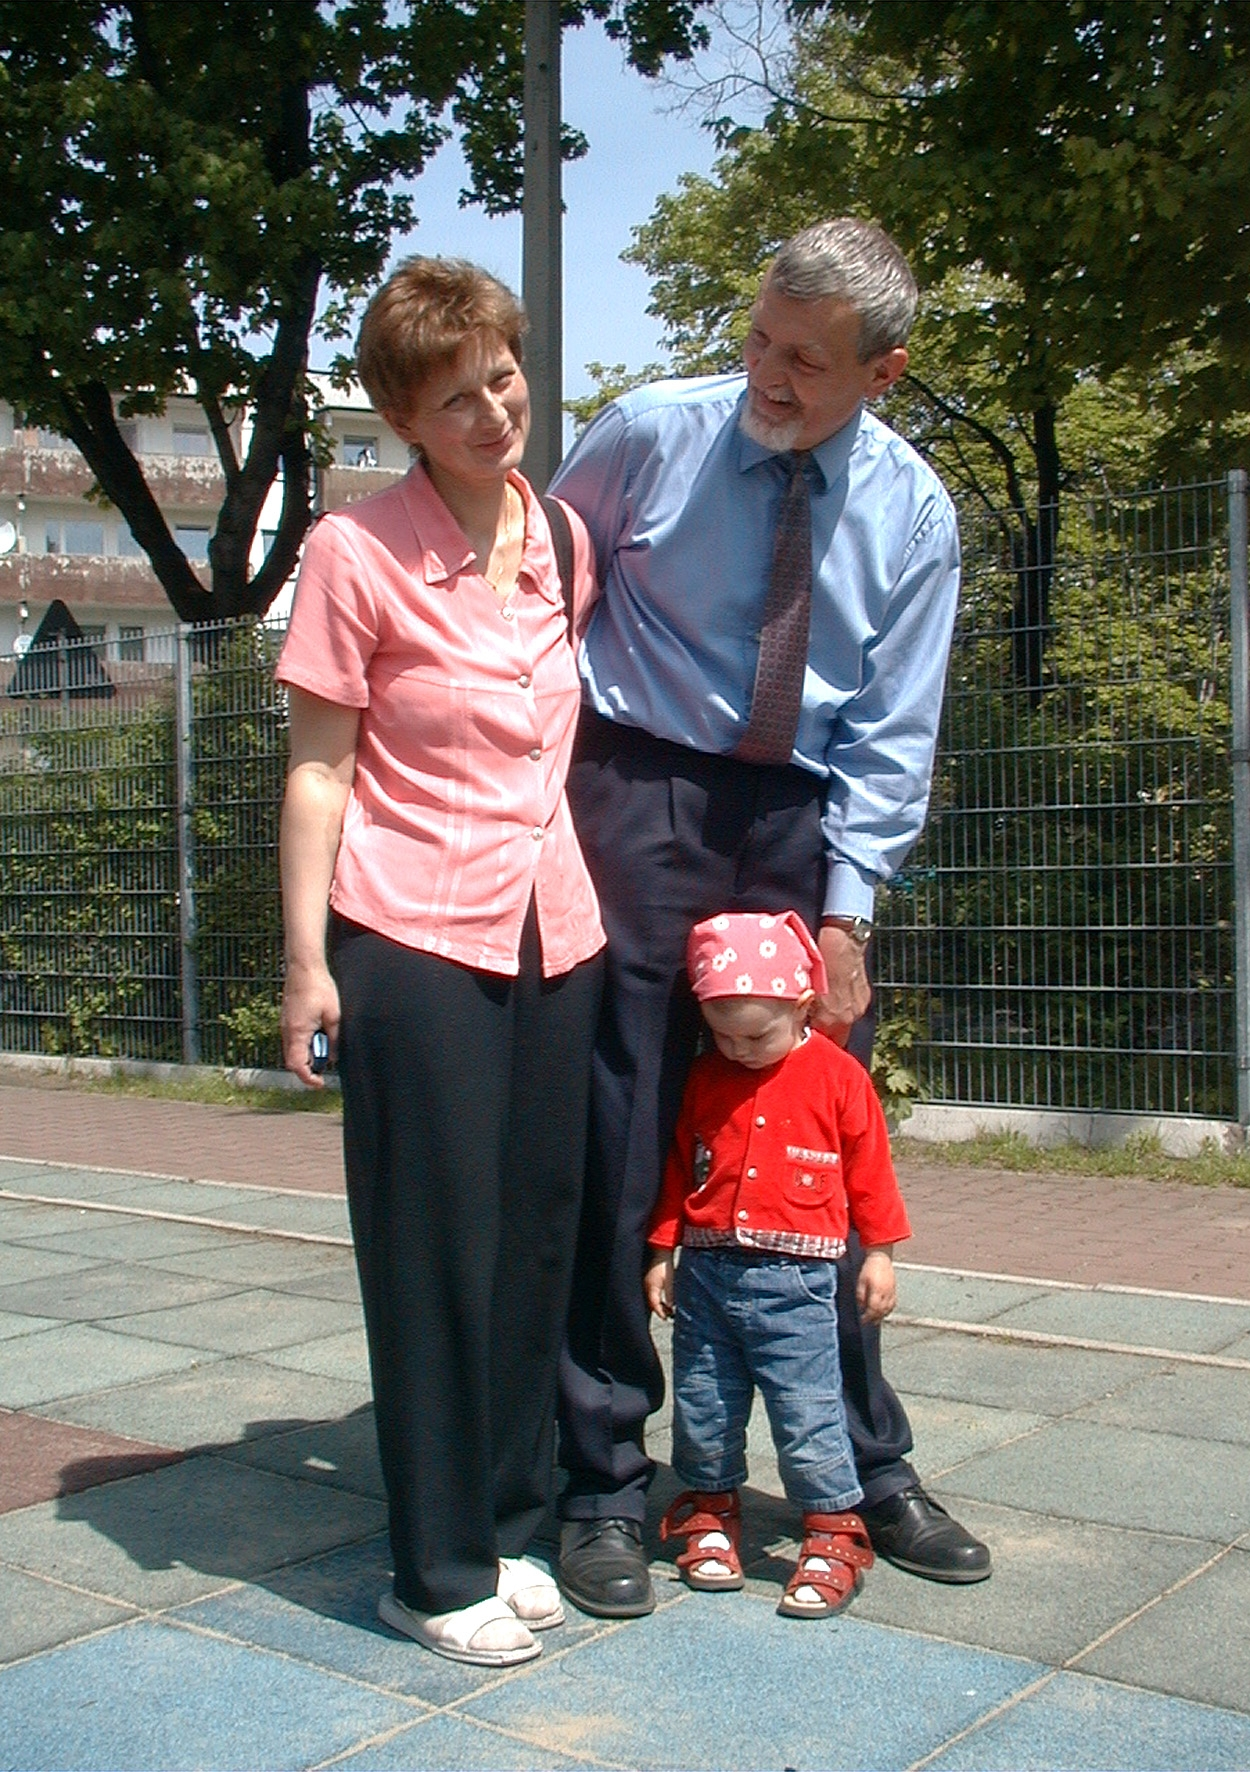
\includegraphics[height=70mm]{photo/malgorzata_sojka.jpg}
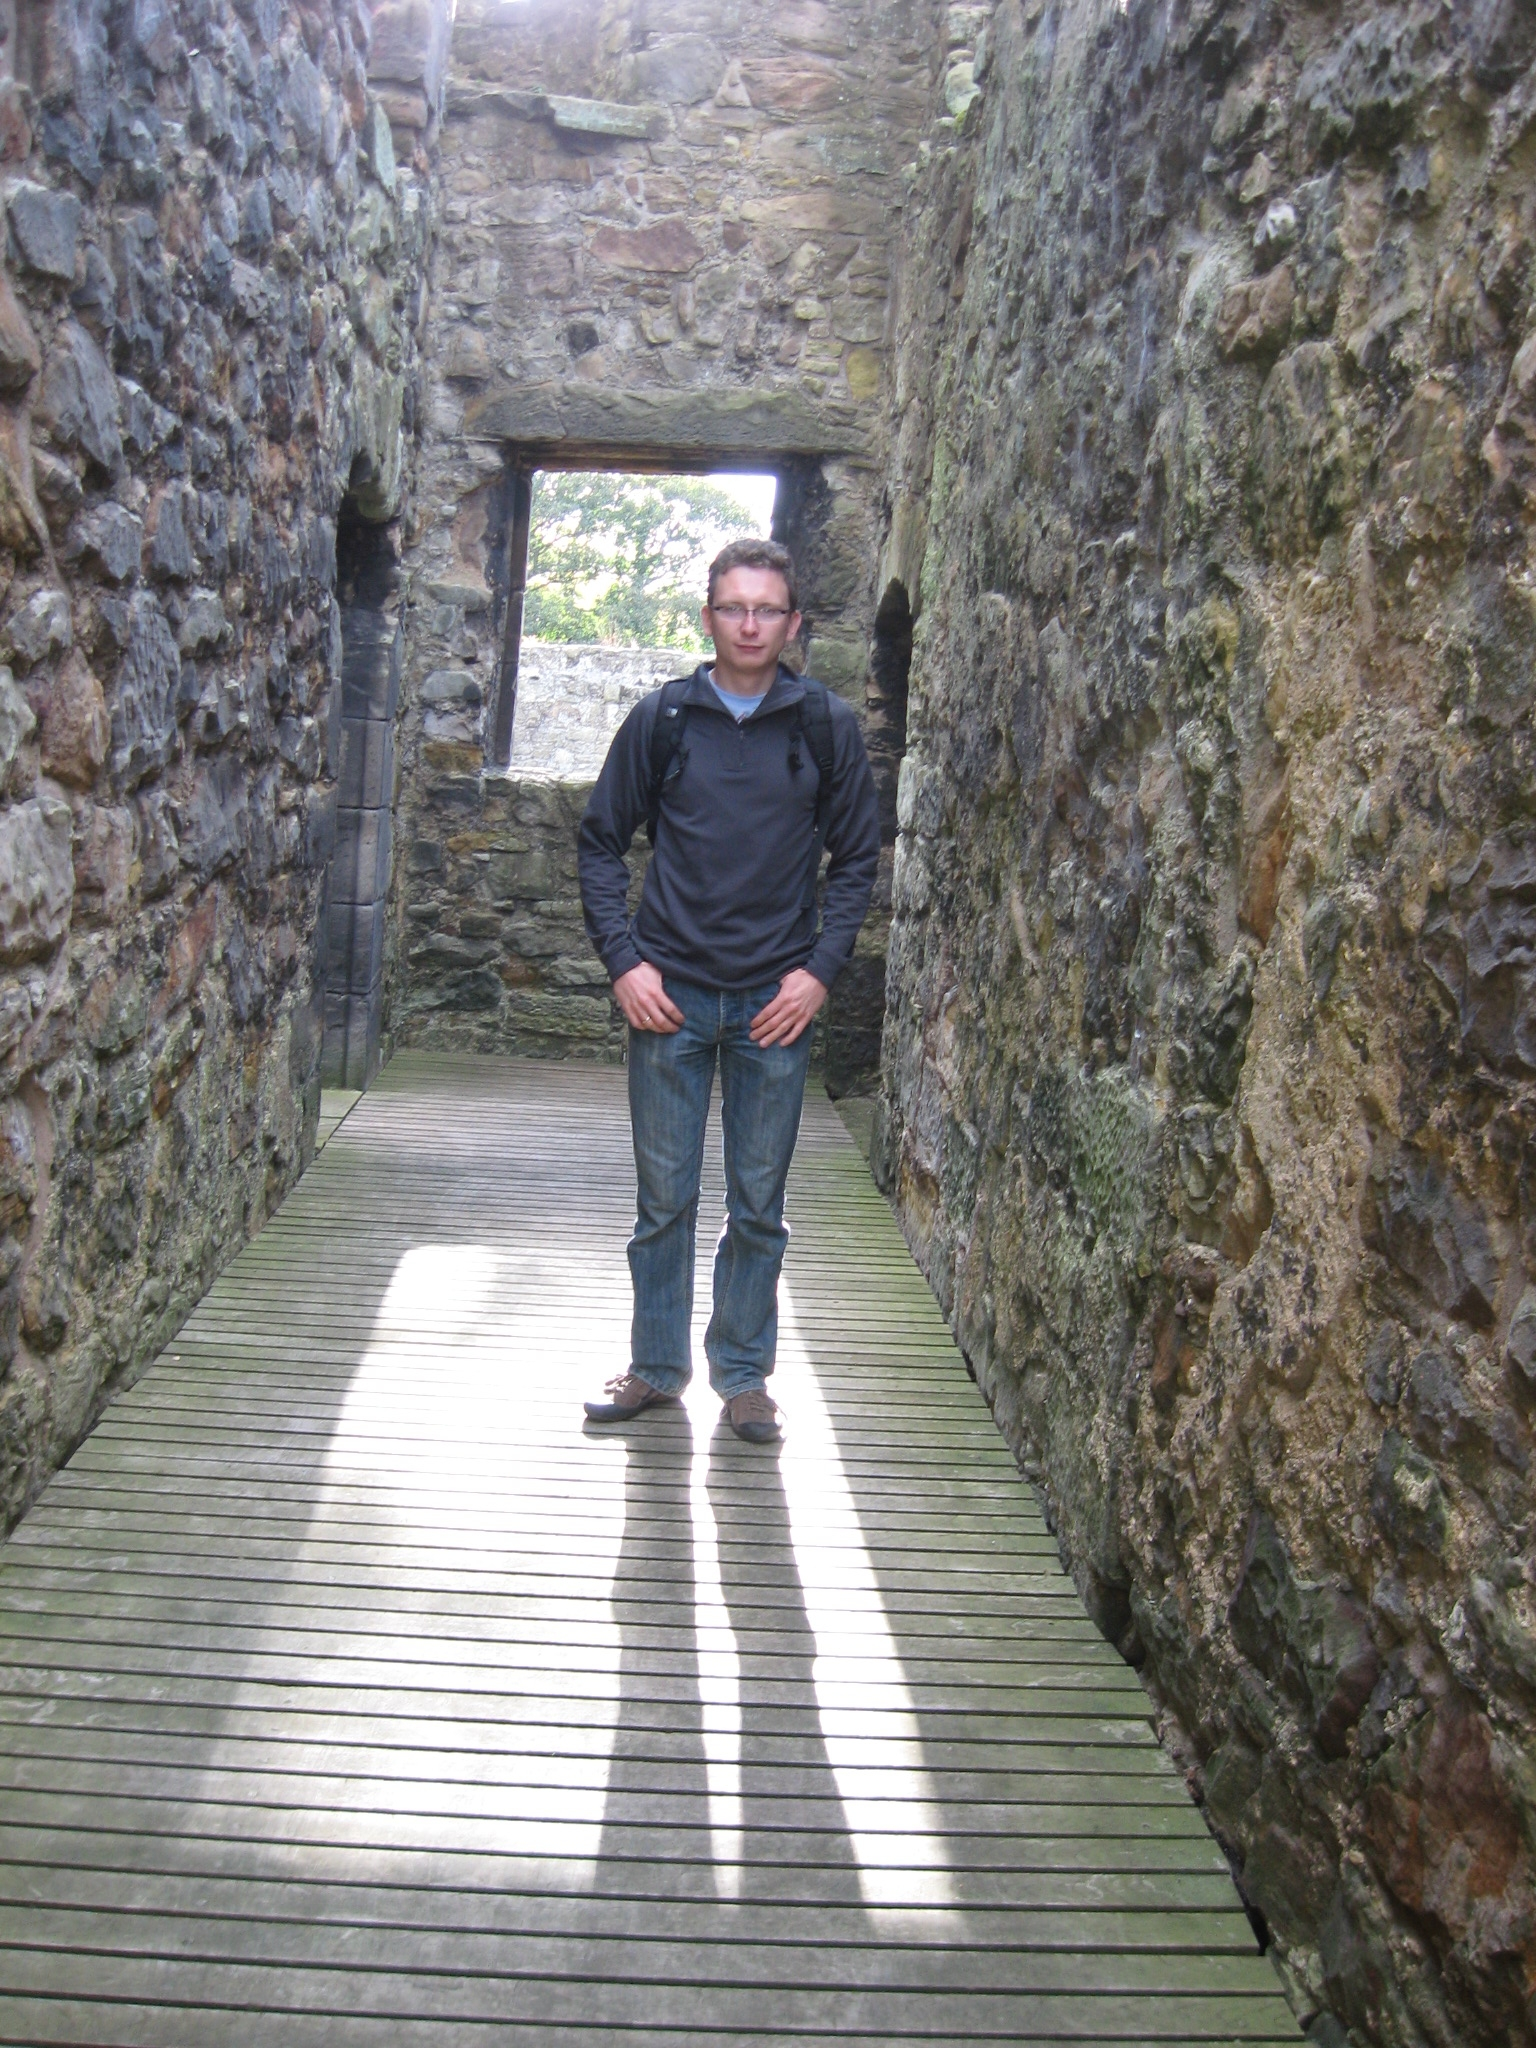
\includegraphics[height=70mm]{photo/bozydar_swierczynski_2.jpg}
\caption{Małgorzata Sojka i Bożydar Świerczyński}
\end{center}
\end{figure}






